% \section{Additional experiments}\label{sec:additional-results}
% \subsection{Results for Adult Income}\label{sec:adult-results}
% \begin{figure*}[htp]
%     \centering
%     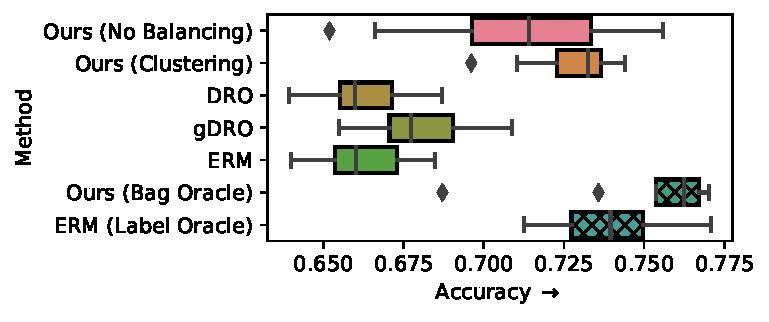
\includegraphics[width=0.49\textwidth]{supmatch/figures/adult/subgroup_bias/adult_partial_acc.pdf}
%     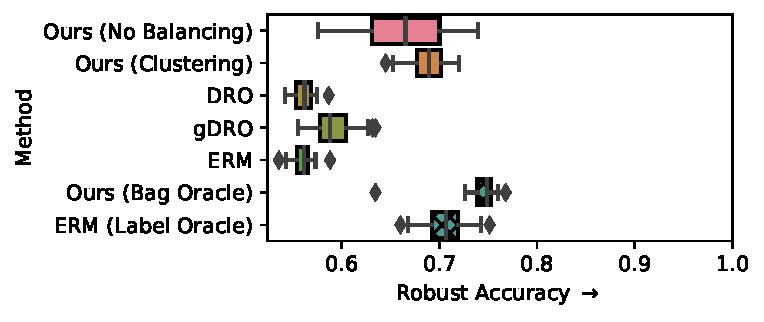
\includegraphics[width=0.49\textwidth]{supmatch/figures/adult/subgroup_bias/adult_partial_acc-min.pdf}
%     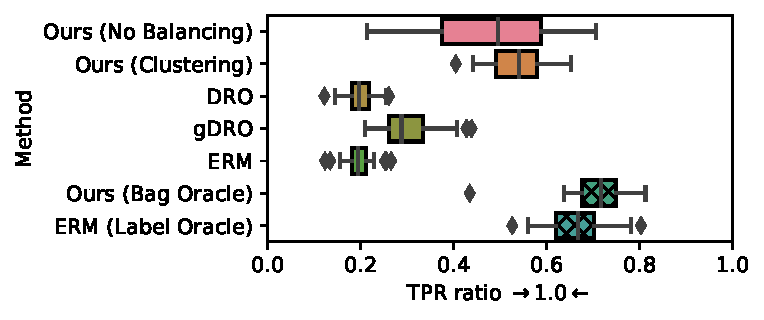
\includegraphics[width=0.49\textwidth]{supmatch/figures/adult/subgroup_bias/adult_partial_tprr.pdf}
%     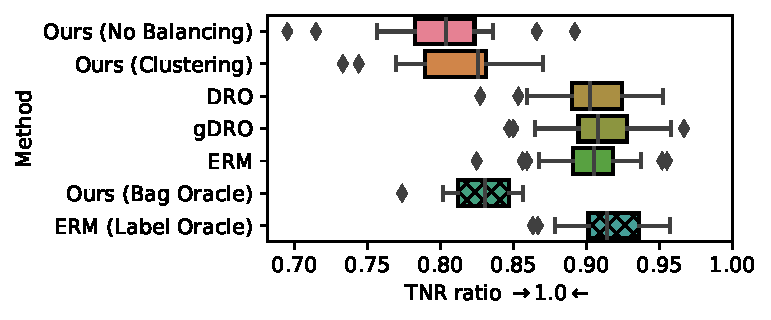
\includegraphics[width=0.49\textwidth]{supmatch/figures/adult/subgroup_bias/adult_partial_tnrr.pdf}
%     \caption{%
%     Results for the Adult Income dataset with \emph{subgroup bias}, for the binary classification
%     task of predicting whether an individual earns $>$\$50,000 with a binary subgrouping based on
%     \emph{gender}. \texttt{ERM (Label Oracle)} refers to a model based on ERM (empirical risk
%     minimization), trained on a labeled deployment set and as such not suffering from bias
%     present in the training set.
%     \textbf{Top left}: Accuracy.
%     \textbf{Top right}: Robust Accuracy.
%     \textbf{Bottom left}: True positive rate ratio.
%     \textbf{Bottom right}: True negative rate ratio.
%     For \texttt{Ours (Clustering)}, the clustering accuracy was 69.7\% $\pm$ 0.3\%;
%     % for \texttt{K-means} it was 43\% $\pm$ 3\%.
%     }%
%     \label{fig:adult-subgroup-bias}
% \end{figure*}
% \begin{figure*}[htp]
%     \centering
%     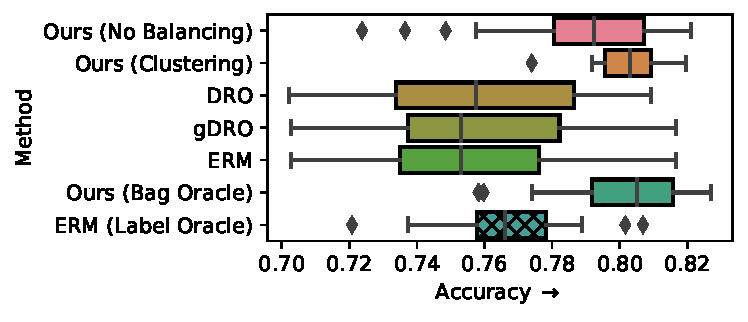
\includegraphics[width=0.49\textwidth]{supmatch/figures/adult/missing_subgroup/adult_miss_s_acc.pdf}
%     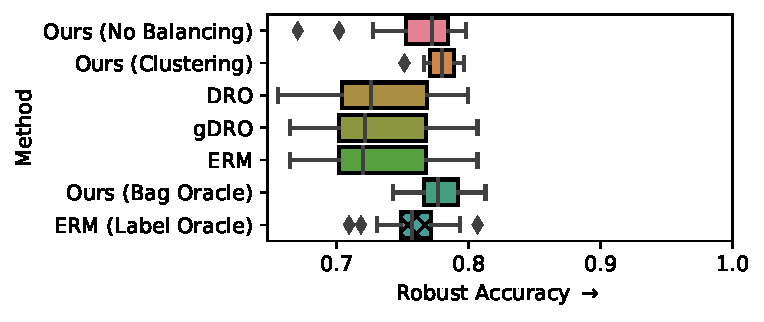
\includegraphics[width=0.49\textwidth]{supmatch/figures/adult/missing_subgroup/adult_miss_s_acc-min.pdf}
%     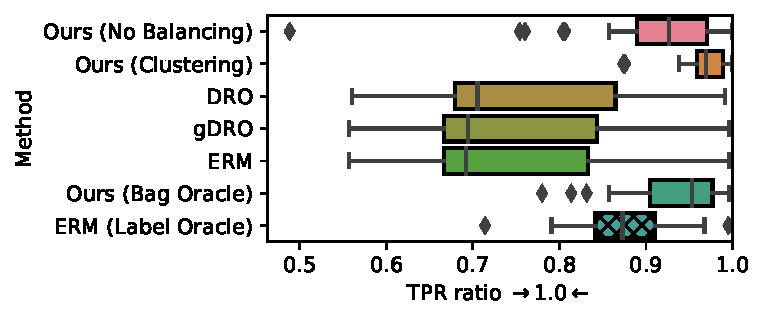
\includegraphics[width=0.49\textwidth]{supmatch/figures/adult/missing_subgroup/adult_miss_s_tprr.pdf}
%     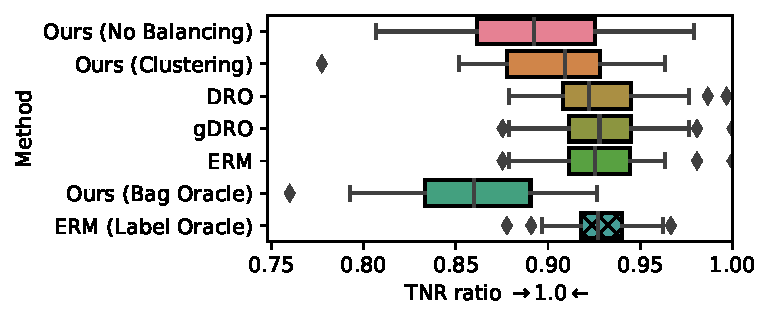
\includegraphics[width=0.49\textwidth]{supmatch/figures/adult/missing_subgroup/adult_miss_s_tnrr.pdf}
%     \caption{%
%     Results for the Adult Income dataset with a \emph{missing subgroup}, for the binary
%     classification task of predicting whether an individual earns $>$\$50,000 with a binary
%     subgrouping based on \emph{gender}.
%     \texttt{ERM (Label Oracle)} refers to a model based on ERM (empirical risk minimization),
%     trained on a \textbf{l}abeled \textbf{d}eployment set; thus not suffering from bias in the training set.
%     \textbf{Top left}: Accuracy.
%     \textbf{Top right}: Robust Accuracy.
%     \textbf{Bottom left}: True positive rate ratio.
%     \textbf{Bottom right}: True negative rate ratio.
%     For\texttt{Ours (Clustering)}, the clustering accuracy was 60.4\% $\pm$ 0.8\%.
%     % for \texttt{K-means} it was 44\% $\pm$ 3\%.
%     }%
%     \label{fig:adult-missing-subgroup}
% \end{figure*}
% Figures~\ref{fig:adult-subgroup-bias} and \ref{fig:adult-missing-subgroup} show results from our
% method on the Adult Income dataset \cite{Dua:2017}. This dataset is a common dataset for
% evaluating fair machine learning models. Each instance in the dataset is described by $14$
% characteristics including gender, education, marital status, number of work hours per week among
% others, along with a label denoting income level ($\geq$\$50K or not). We transform the
% representation into $62$ real and binary features along with the subgroup label $s$.
% %%%%%%%%CHECK THESE VALUES%%%%%%%%%%%% The dataset is naturally imbalanced with respect to
% gender: 30\% of the males are labeled as earning more than \$50K per year (high income), while
% only 11\% of females are labeled as such. For further details on the dataset construction, see
% section~\ref{ssec:dataset-construction-adult}. % Following standard practice in algorithmic
% fairness  e.g. \cite{ZemeWuSwePitetal13}, we consider gender to be the subgroup label $s$. % A
% \emph{source} is defined as certain combinations of the subgroup, $s$, and target class, $y$.

% For the Adult Income dataset, we study the following two settings of missing sources, a subgroup
% bias setting and a more extreme missing subgroup setting: 1) \emph{subgroup bias}: we have
% labeled training data for males ($s=1$) with both positive and negative outcomes, but for the
% group of females ($s=0$), we only observe the one-sided negative outcome:
% \(\mathcal{S}_{tr}(y=1)=\{1\}\); 2) \emph{missing subgroup}: we have training data for males with
% positive and negative outcomes, but do not have labeled data for females, i.e.\
% \(\mathcal{S}_{tr}(y=0)=\{1\}\) and \(\mathcal{S}_{tr}(y=1)=\{1\}\).

% As before, \texttt{Ours (Clustering)}, \texttt{Ours (No Balancing)}\ and \texttt{Ours (Bag
% Oracle)} denote variants of our method with different deployment-set balancing strategies. As
% baseline methods, we have \texttt{ERM} (standard empirical risk minimization with balanced
% batches), \texttt{DRO} \cite{HasSriNamLia18}, \texttt{gDRO} \cite{sagawa2019distributionally} and
% \texttt{ERM (Label Oracle)} which is the same model as \texttt{ERM}, but trained with access to
% the ground-truth labels of the deployment set.

% In both settings, we observe the same order as for the other dataset in terms of accuracy:
% \texttt{Ours (Bag Oracle)} achieves the highest performance, followed by \texttt{Ours
% (Clustering)}, then \texttt{Ours (No Balancing)}. However, for the \emph{missing subgroup}
% setting, \texttt{Ours (Clustering)} and \texttt{Ours (Bag Oracle)} perform almost identically,
% with the former outstripping the latter slightly in terms of de-biasing metrics. This reduced
% reliance on balancing can be explained by the additional supervision that comes with having two
% sources missing instead of one -- in order for the discriminator to distinguish between bags from
% the deployment set and bags from the training set, the former need only contain \emph{one} of the
% two missing sources.

% Generally, we observe a high variance in the results. This is not attributable to our method,
% however, with the baselines exhibiting the same behavior, but rather to the fact that the Adult
% Income dataset is a very noisy dataset which, at the best of times, allows only about 85\%
% accuracy to be attained (see also \cite{agrawal2020debiasing}). The problem is that samples vary
% widely in how informative they are. This, coupled with us artificially biasing the dataset to be
% even more biased (as \emph{subgroup bias} and \emph{missing subgroup}), makes the attainable
% performance very dependent on which samples the classifier gets to see, which varies according to
% the random seed used for the data set split.
%
\subsection{Results for 3-digit 3-colour variant of Coloured MNIST}\label{ssec:3-digit-3-color}
%
To investigate how our method scales with the number of sources, we look to a 3-digit, 3-colour
variant of the dataset in the \emph{subgroup bias} setting where four sources are missing from
$\gD^{tr}$.
Results for this configuration are shown in Fig.~\ref{fig:cmnist-3dig-4miss}. We see that the
performance of \texttt{Ours (No Balancing)} is quite close to that of \texttt{Ours (Bag Oracle)}.
We suspect this is because balancing is less critical with the increased number of subgroups
strengthening the training signal. As inter-subgroup ratios do not make for suitable metric for
non-binary $S$, we instead quantify the invariance of the predictions to the subgroup with the
\ac{HGRMC} \citep{renyi1959measures}.

\begin{figure*}[htp]
  \centering
  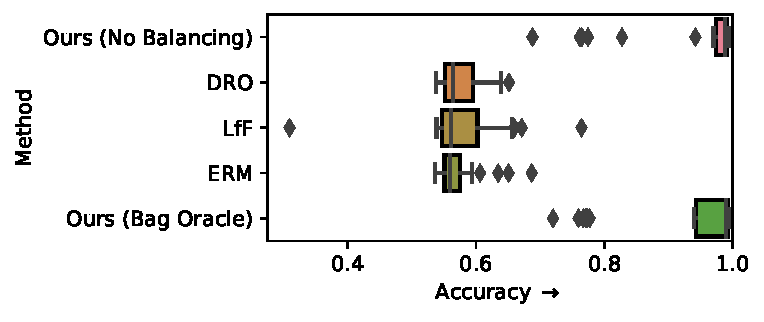
\includegraphics[width=0.49\textwidth]{supmatch/figures/cmnist/supmat/cmnist_3dig_4miss_acc.pdf}
  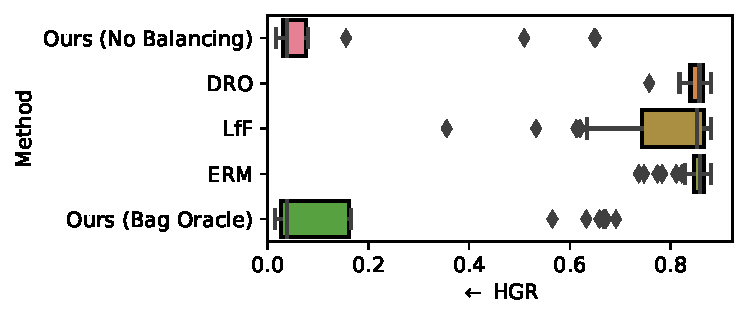
\includegraphics[width=0.49\textwidth]{supmatch/figures/cmnist/supmat/cmnist_3dig_4miss_hgr.pdf}
%   \includegraphics[width=\columnwidth]{supmatch/figures/cmnist_3dig_4miss_pr.pdf}
%   \includegraphics[width=\columnwidth]{supmatch/figures/cmnist_3dig_4miss_tpr.pdf}
%   \includegraphics[width=\columnwidth]{supmatch/figures/cmnist_3dig_4miss_tnr.pdf}
  \caption{
    Results from \textbf{30 repeats} for the Coloured MNIST dataset with three digits: `2', `4' and
    `6'. Four combinations of digit and colour are missing: {\color{green}green} 2's,
    {\color{blue}blue} 2's, {\color{blue}blue} 4's and {\color{green}green} 6's. \textbf{Left}:
    Accuracy. \textbf{Right}: Hirschfeld-Gebelein-R\'enyi maximal correlation
    \cite{renyi1959measures} between $S$ and $Y$.
  }%
  \label{fig:cmnist-3dig-4miss}
\end{figure*}
%
\subsection{Extended Results for CelebA}\label{ssec:extended-results-celeba}
%
As alluded to in main text, for three out of four of the missing gender/smiling quadrants, the
\texttt{GEORGE} baseline produced an extreme outlier for one out of the five total repeats - these
outliers were omitted from the plots to ensure the discriminability of the other results.
%
We reproduce the full, untruncated versions of these plots here in
Fig.~\ref{fig:celeba-gender-smiling-full}. We have also included \texttt{Accuracy} metric in
Fig.~\ref{fig:celeba-gender-smiling-full}.


\begin{figure*}[htp]
  \centering
  % Smiling females missing
%   \normalsize{Missing source: smiling females}\par\medskip
 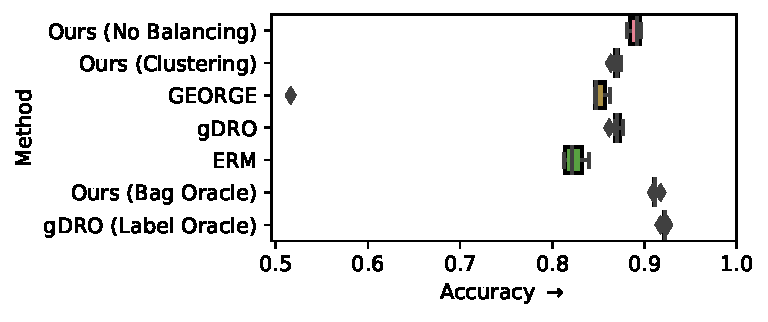
\includegraphics[width=0.49\textwidth]{supmatch/figures/celeba/supmat/no_smiling_females/celeba_gender_smiling_acc.pdf}
  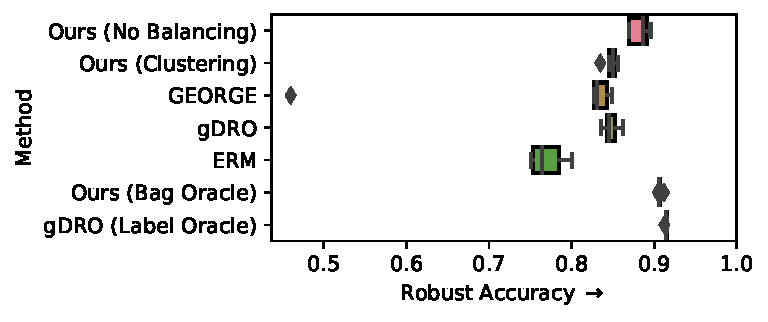
\includegraphics[width=0.49\textwidth]{supmatch/figures/celeba/supmat/no_smiling_females/celeba_gender_smiling_acc-min.pdf}
    % Smiling males missing
%   \normalsize{Missing source: smiling males}\par\medskip
 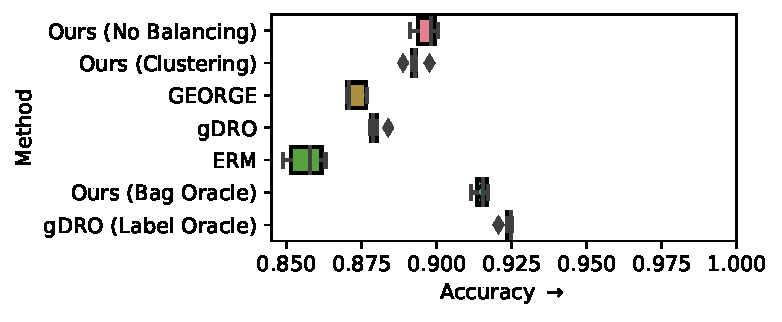
\includegraphics[width=0.49\textwidth]{supmatch/figures/celeba/supmat/no_smiling_males/celeba_gender_smiling_acc.pdf}
 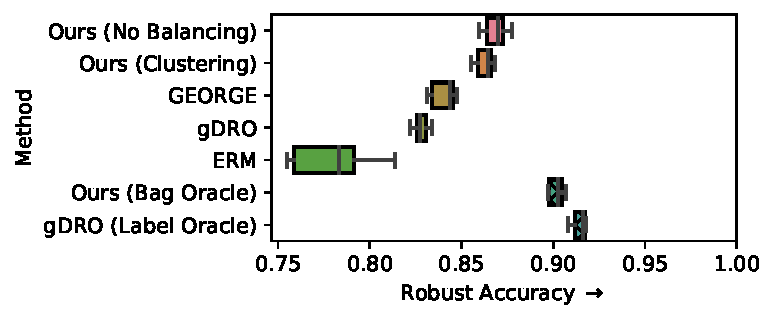
\includegraphics[width=0.49\textwidth]{supmatch/figures/celeba/supmat/no_smiling_males/celeba_gender_smiling_acc-min.pdf}
    % Unsmiling females missing
%   \normalsize{Missing source: non-smiling} females\par\medskip
 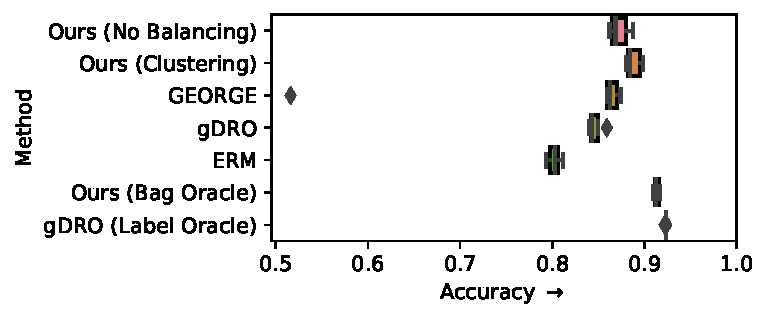
\includegraphics[width=0.49\textwidth]{supmatch/figures/celeba/supmat/no_unsmiling_females/celeba_gender_smiling_acc.pdf}
  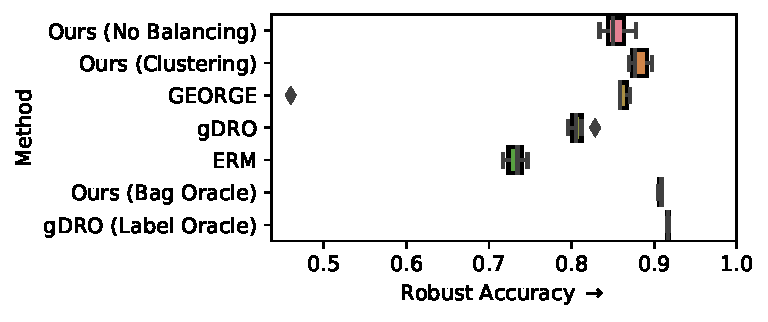
\includegraphics[width=0.49\textwidth]{supmatch/figures/celeba/supmat/no_unsmiling_females/celeba_gender_smiling_acc-min.pdf}
  % Unsmiling males missing
%   \normalsize{Missing source: non-smiling males}\par\medskip
 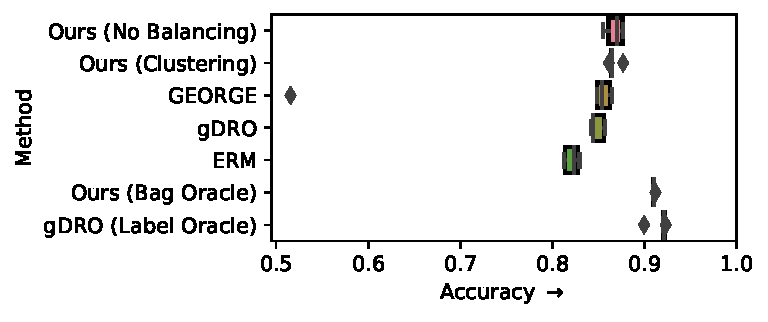
\includegraphics[width=0.49\textwidth]{supmatch/figures/celeba/supmat/no_unsmiling_males/celeba_gender_smiling_acc.pdf}
  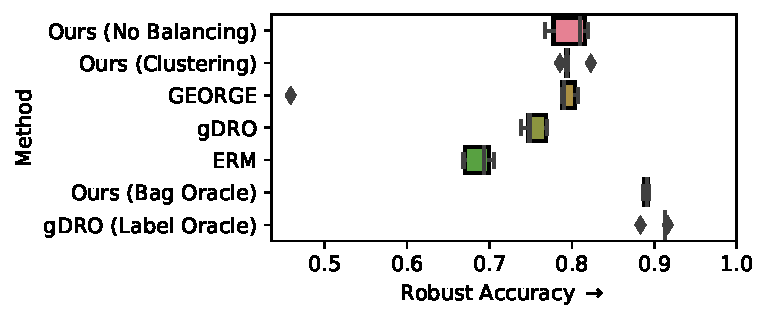
\includegraphics[width=0.49\textwidth]{supmatch/figures/celeba/supmat/no_unsmiling_males/celeba_gender_smiling_acc-min.pdf}
\caption{
    Results from \textbf{5 repeats} for the CelebA dataset for the \emph{subgroup bias} scenario.
    The task is to predict ``smiling'' vs ``non-smiling'' and the subgroups are based on gender.
    The four sources are dropped one at a time from the training set
    (\textbf{first row}: smiling females; \textbf{second row}: smiling males; \textbf{third row}:
    non-smiling females, \textbf{fourth row}: non-smiling males), while the deployment set is kept
    fixed. ``Robust Accuracy'' refers to the minimum accuracy computed over the subgroups. 
  }%
 \label{fig:celeba-gender-smiling-full}
\end{figure*}

\section{Theoretical analysis}\label{sec:sm-theoretical-analysis}
%
In this section, we present our theoretical results concerning the validity of our support-matching
objective and the bound on the error introduced into it by clustering. 
%
We use notation consistent with that used throughout the main text.

\subsection{Sampling function for the objective}%
\label{sub:sampling_function_for_objective}
The stated objective uses the following helper function:
\begin{align}
\Pi(s',y') = \begin{cases}
  \{s'\}&\text{if }\,\gS^{tr}_{Y=y\prime}=\gS\\
  \gS^{tr}_{Y=y'}&\text{otherwise}~.
\end{cases}
\end{align}
This helper function determines which $s$ value in the training set an $s$-$y$ pair from the
deployment set is mapped to. (The $y$ value always stays \emph{the same} when mapping from
deployment set to training set.) To demonstrate the usage of this function, we consider the example
of binary Coloured MNIST with \(\gS=\{\text{\color{purple}{purple}}, \text{\color{green}green}\}\)
and \(\gY=\{2, 4\}\) where the training set is missing \((s=\text{purple}, y=4)\). In this case,
$\Pi$ takes on the following values:
\begin{align}
  \Pi(\text{{\color{purple}purple}}, 2) &= \{\text{\color{purple}purple}\}\\
  \Pi(\text{\color{green}green},  2) &= \{\text{\color{green}green} \}\\
  \Pi(\text{\color{purple}purple}, 4) &=\gS^{tr}_{y=4} = \{\text{\color{green}green} \}\\
  \Pi(\text{\color{green}green},  4) &=\gS^{tr}_{y=4} = \{\text{\color{green}green} \}
\end{align}
% See also figure \ref{fig:matching-repeated} which is a visualization of this.
It is essential that \((s=\text{\color{purple}{purple}}, y=4)\) from the deployment set is mapped
to \((s=\text{\color{green}{green}}, y=4)\) from the training set, and not
\((s=\text{\color{purple}{purple}}, y=2)\).
% The latter would produce an invariance to $y$, which is undesirable.
This procedure is illustrated in Fig.~\ref{fig:matching-repeated-correct}, and contrasted with an
incorrect procedure based on balancing the bag according to $s$ in
\ref{fig:matching-repeated-incorrect} -- such a procedure would result in invariance to $y$ instead
of $s$, which is obviously undesirable.

In practice, we use the following sampling function $\pi$ to implement $\Pi$, sampling from it for
all $(s,y) \in S \times Y$:
%
\begin{align}
  \pi(s',y') = \begin{cases} x\sim P^\mathit{tr}(x|S=s',y'), \\
    \quad\quad\quad\quad\quad\quad\quad\quad\text{if }\,\gS^{tr}_{Y=y'}=\gS \\
  x\sim P^\mathit{tr}(x|s=\check{s},y'), \check{s}\sim \mathrm{uniform}(S^{tr}), \\
    \quad\quad\quad\quad\quad\quad\quad\quad\text{otherwise}~.
\end{cases}
\label{eq:functional-sampling}
\end{align}
%
With the assumption that our data follows a two-level hierarchy and all digits appear in the
training set, the above sampling function $\pi$ traverses the first level which corresponds to the
class-level information, and \emph{samples} the second level which corresponds to subgroup-level
information when we have missing sources.
 
% ensures that the bags from the training set only differ from those from the deployment set where
% a source is missing; and furthermore, that they only differ in $s$, but not in $y$.

\begin{figure}[htp]
  \begin{subfigure}{0.49\textwidth}
    \centering
    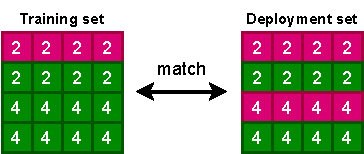
\includegraphics[width=0.9\linewidth]{supmatch/figures/illustrations/matching_diagram.pdf}
    \caption{Correct matching procedure.}%
    \label{fig:matching-repeated-correct}
  \end{subfigure}
  \begin{subfigure}{0.49\textwidth}
    \centering
    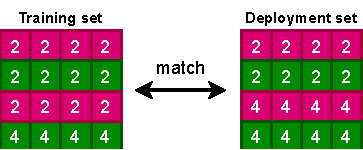
\includegraphics[width=0.9\linewidth]{supmatch/figures/illustrations/y-inv.pdf}
    \caption{\emph{In}correct matching procedure.}%
    \label{fig:matching-repeated-incorrect}
  \end{subfigure}
  \caption{%
    The two natural matching procedures for one missing source in the training set.
    Only figure \ref{fig:matching-repeated-correct} (left) produces the desired invariance.
  }%
  \label{fig:matching-repeated}
\end{figure}


% Sampling from $\pi (s,y)$ for all $(s,y) \in S \times Y$ ensures that the bags from the training
% set only differ from those from the deployment set where a source is missing; and furthermore,
% that they only differ in $s$, but not in $y$. For example, if the bag size is four, $\gY$ and
% $\gS$ are binary, and the combination $(y=1,s=0)$ is missing, then each bag should contain two
% samples of $(y=1,s=1)$ and one sample each for $(y=0,s=0)$ and $(y=0,s=1)$. e.

\subsection{Implication of the objective}\label{implication-of-the-objective}
We restate proposition 1 and present the proof.

We prove here that an encoding $f$ satisfying the objective is invariant to \(s\), at least in
those cases where the class does not have full \(s\)-support (which is exactly the case where it
matters).

\begin{theorem}
If \(f\) is such that
\begin{align}
p_f|_{s\in \Pi(s',y'),Y=y'} = q_f|_{S=s',Y=y'}\quad\forall s'\in\gS, y' \in\gY
\end{align}
%
and \(P^\mathit{tr}\) and \(P^\mathit{dep}\) are data distributions that correspond to the real
data distribution \(P\), except that some \(s\)-\(y\)-combinations are less prevalent, or, in the
case of \(P^\mathit{tr}\), missing entirely, then, for every \(y'\in\gY\), there is either full
coverage of \(s\) for \(y'\) in the training set (\(\gS^{tr}_{Y=y\prime}=\gS\)), or the following
holds:
%
\begin{align}
P(S=s'|f(X)=z', Y=y')=\frac{1}{n_s}~.
\end{align}
%
In other words: for \(Y=y'\), \(f(x)\) is not predictive of \(s\).
\end{theorem}

\begin{proof}
If \(y'\) has full coverage of \(s\) in the training set, there is nothing to prove.
%
So, assume \(y'\) does not have full \(s\)-support.
%
That means \(\Pi(s',y')=\gS^{tr}_{Y=y\prime} \) for all \(s'\in \gS\).
%
And so
%
\begin{align}
&P^\mathit{tr}(f(X)=z'|s\in \gS^{tr}_{Y=y\prime}, Y=y')\\
  =\;&P^\mathit{dep}(f(X)=z'|S=s', Y=y')\quad\quad\quad\quad\forall s'\in\gS \nonumber
\end{align}
%
The left-hand side of this equation does not depend on \(s'\)
and so the right-hand side must have the same value for all \(s'\in\gS\), which implies:
\begin{align}
&P^\mathit{dep}(f(X)=z'|S=s', Y=y') \nonumber\\
  =\;&P^\mathit{dep}(f(X)=z'|Y=y')
\end{align}
%
Now, by assumption, the different data distributions \emph{train} and \emph{deployment} only differ
from the ``true'' distribution by the prevalence of the different \(s\)-\(y\)-combinations, with
the \emph{deployment} data distribution having all combinations but potentially not in equal
quantity. However, as we restrict ourselves to a certain combination (\(S=s',Y=y'\)) in the above
equation, the equation also holds in the true data distribution:
%
\begin{align}
&P(f(X)=z'|S=s', Y=y') \nonumber\\
=\;&P(f(X)=z'|Y=y')
\end{align}
%
Then, using Bayes' rule, we get
%
\begin{align}
&P(S=s'|f(X)=z', Y=y') \nonumber\\
=\;&\frac{P(f(X)=z'|S=s', Y=y')P(S=s'|Y=y')}{P(f(X)=z'|Y=y')} \nonumber\\
=\;&P(S=s'| Y=y')~.
\end{align}
%
Finally, in the true data distribution, we have a uniform prior:
\(P(S=s'|Y=y')=(n_s)^{-1}\). This concludes the proof.
\end{proof}
%
\subsection{Bound on error introduced by clustering}\label{bound-on-error-introduced-by-clustering}
%
As previously stated, in practice, no labels are available for the deployment set.
Instead, we identify the relevant groupings by clustering.
Such clustering cannot be expected to be perfect.
So, how will clustering affect the calculation of our objective?

\begin{theorem}
  %
If \(q_f(Z)\) is a data distribution on \(\mathcal{Z}\) that is a mixture of \(n_y\cdot n_s\)
Gaussians, which correspond to all unique combinations of \(y\in\gY\) and \(s\in\gS\), and
\(p_f(Z)\) is any data distribution on \(\mathcal{Z}\), then without knowing \(y\) and \(s\) on
\(q_f\), we can estimate
%
\begin{align}
\sum\limits_{s'\in\gS}\sum\limits_{y'\in\gY} TV(p_f|_{s\in \Pi(s',y'),Y=y'}, q_f|_{S=s',Y=y'})
\end{align}
%
with an error that is bounded by \(\tilde{O}(\sqrt{1/N})\) with high probability, where \(N\) is
the number of samples drawn from \(q_f\) for learning.
%
\end{theorem}

\begin{proof}
First, we produce an estimate \(\hat{q}_f\) of \(q_f\) using the algorithm from
\citet{ashtiani2020near}, which gives us a mixture-of-Gaussian distribution of \(n_y\cdot n_s\)
components with \(TV(q_f, \hat{q}_f)\leq \tilde{O}(\sqrt{1/N})\) with high probability, where \(N\)
is the number of data points used for learning the estimate. Then, by Lemma 3 from
\citet{SohDunAngGuetal20}, \emph{there exists} a mapping \(i\) from the components \(k\) of the
Gaussian mixture \(\hat{q}_f\) to the \(s\)-\(y\)-combinations in \(q_f\) such that
%
\begin{align}
&TV(q_f(Z|S=s',Y=y'),\hat{q}_f(Z|k=i(s',y'))) \\
&\quad\quad\quad\quad\quad\quad\quad\quad\quad\quad\quad\quad\quad\quad\leq
\tilde{O}\left(\frac{1}{\sqrt{N}}\right)~. \nonumber
\end{align}
%
Now, consider the element of the sum in the objective that corresponds
to \((s',y')\):
%
\begin{align}
&TV(p_f(Z|s\in \Pi(s',y'),Y=y'), q_f(z|S=s',Y=y'))\nonumber\\
\leq \;&TV(p_f(Z|s\in \Pi(s',y'),Y=y'), \hat{q}_f(Z|k=i(s',y')))\nonumber\\
&\quad\quad+TV(\hat{q}_f(z|k=i(s',y')), q_f(z|S=s',Y=y'))\nonumber\\
\leq \;&TV(p_f(Z|s\in \Pi(s',y'),Y=y'), \hat{q}_f(Z|k=i(s',y'))) \nonumber\\
&\quad\quad+\tilde{O}(1/\sqrt{N})
\end{align}
%
Thus, for the whole sum over \(s\) and \(y\), the error is bounded by
\begin{align}
\sum\limits_{s'\in\gS}\sum\limits_{y^\prime\in\gY}\tilde{O}(\sqrt{1/N})
\leq n_sn_y \max\limits_{(s',y')\in\gS\times\gY}\tilde{O}(\sqrt{1/N})
\end{align}
which is equivalent to just \(\tilde{O}(\sqrt{1/N})\).
\end{proof}
%
\section{Dataset Construction}\label{sec:dataset-construction}
%
\subsection{Coloured MNIST and biasing parameters}
%
The MNIST dataset \citep{lecun1998gradient} consists of 70,000 (60,000 designated for training,
10,000 for testing) images of grey-scale hand-written digits. We colour the digits following the
procedure outlined in \citet{KehBarThoQua20}, randomly assigning each sample one of ten distinct RGB
colours. Each source is then a combination of digit-class (class label) and colour (subgroup label).
We use no data-augmentation aside from symmetrically zero-padding the images to be of size 32x32.
% To simulate a more realistic setting, we create artificial imbalance in both $\gD_{dep}$ and
% $\gD^{tr}$ by sub-sampling the remaining sources. 
%The sub-sampling proportions used for each set of experiments can be found in Appendix E.

%\subsection{Coloured MNIST biasing parameters}
To simulate a more real-world setup where the data, labelled or otherwise, is not naturally
balanced, we bias the Coloured MNIST training and deployment sets by downsampling certain
colour/digit combinations. The proportions of each such combination \emph{retained} in the
\emph{subgroup bias} (in which we have one source missing from the training set) and \emph{missing
subgroup} (in which we have two sources missing from the training set) are enumerated in
table~\ref{color_mnist_biasing_po} and \ref{color_mnist_biasing_id}, respectively. For the
3-digit-3-colour variant of the problem, no biasing is applied to either the deployment set or the
training set (the missing combinations are specified in the caption accompanying
figure~\ref{fig:cmnist-3dig-4miss-add}); this variant was experimented with only under the
subgroup-bias setting.

\begin{table}[ht]
\caption{Biasing parameters for the training (left) and deployment (right) sets of Coloured MNIST in
the \emph{subgroup bias} setting.}
\label{color_mnist_biasing_po}
\centering
\begin{tabular}{lcc}
\toprule
Combination   & \multicolumn{2}{c}{Proportion retained} \\ \cmidrule(lr){2-3}
  & training set & deployment set \\ \midrule
(Y = 2, S = {\color{purple}purple}) & 1.0  & 0.7 \\
(Y = 2, S = {\color{green}green})   & 0.3  & 0.4 \\
(Y = 4, S = {\color{purple}purple}) & 0.0  & 0.2 \\
(Y = 4, S = {\color{green}green})   & 1.0  & 1.0 \\
\bottomrule
\end{tabular}
\end{table}

\begin{table}[ht]
\caption{Biasing parameters for the training (left) and deployment (right) sets of Coloured MNIST in
the \emph{missing subgroup} setting.}
\label{color_mnist_biasing_id}
\centering
\begin{tabular}{lcc}
\toprule
Combination   & \multicolumn{2}{c}{Proportion retained} \\ \cmidrule(lr){2-3}
  & training set & deployment set \\ \midrule
(Y = 2, S = {\color{purple}purple}) & 0.0  & 0.7 \\
(Y = 2, S = {\color{green}green})   & 0.85 & 0.6 \\
(Y = 4, S = {\color{purple}purple}) & 0.0  & 0.4 \\
(Y = 4, S = {\color{green}green})   & 1.0  & 1.0 \\
\bottomrule
\end{tabular}
\end{table}

% \subsection{Adult Income biasing parameters}\label{ssec:dataset-construction-adult}
% For the Adult Income dataset, we do not need to apply any synthetic biasing as the dataset
% naturally contains some bias \wrt{} $s$. Thus, we instantiate the deployment set as just a random
% subset of the original dataset. However, explicit balancing of the test set \emph{is} needed to
% yield meaningful evaluation (namely through the penalizing of biased classifiers) but care needs
% to be taken in doing so. Balancing the test set such that
% \begin{align}
%     |\{x \in X |s=0, y=0\}| &= |\{x \in X |s=1, y=0\}|    \nonumber\\
%     \text{and}~|\{x \in X |s=0, y=1\}| &= |\{x \in X |s=1, y=1\}|
% \end{align}
% where for both target classes, $y=0$ and $y=1$, the proportions of the groups $s=0$ and $s=1$ are
% made to be the same, is intuitive, yet at the same time precludes sensible comparison of the
% accuracy/fairness trade-off of the different classifiers. Indeed, with the above conditions, a
% majority classifier (predicting all 1s or 0s) achieves comparable accuracy to the
% fairness-unaware baselines, while also being perfectly fair by construction.
% This observation motivated us to devise an alternative scheme, where we balance the test set
% according to the following constraints
% \begin{align}
%     & |\{x \in X |s=0, y=0\}| 
%     = |\{x \in X |s=0, y=1\}|  \nonumber \\
%     = &|\{x \in X |s=1, y=1\}|
%     = |\{x \in X |s=1, y=0\}|~.
%  \end{align}
% That is, all subsets of $\gS \times \gY$ are made to be equally sized. Under this new scheme the
% accuracy of the the majority classifier is 50\% for the binary-classification task.

\section{Model details and optimization}
\subsection{Overview of model architecture}\label{sec:model-arch}
\begin{figure*}[htp]
    % \begin{subfigure}{0.74\textwidth}
    \centering
    %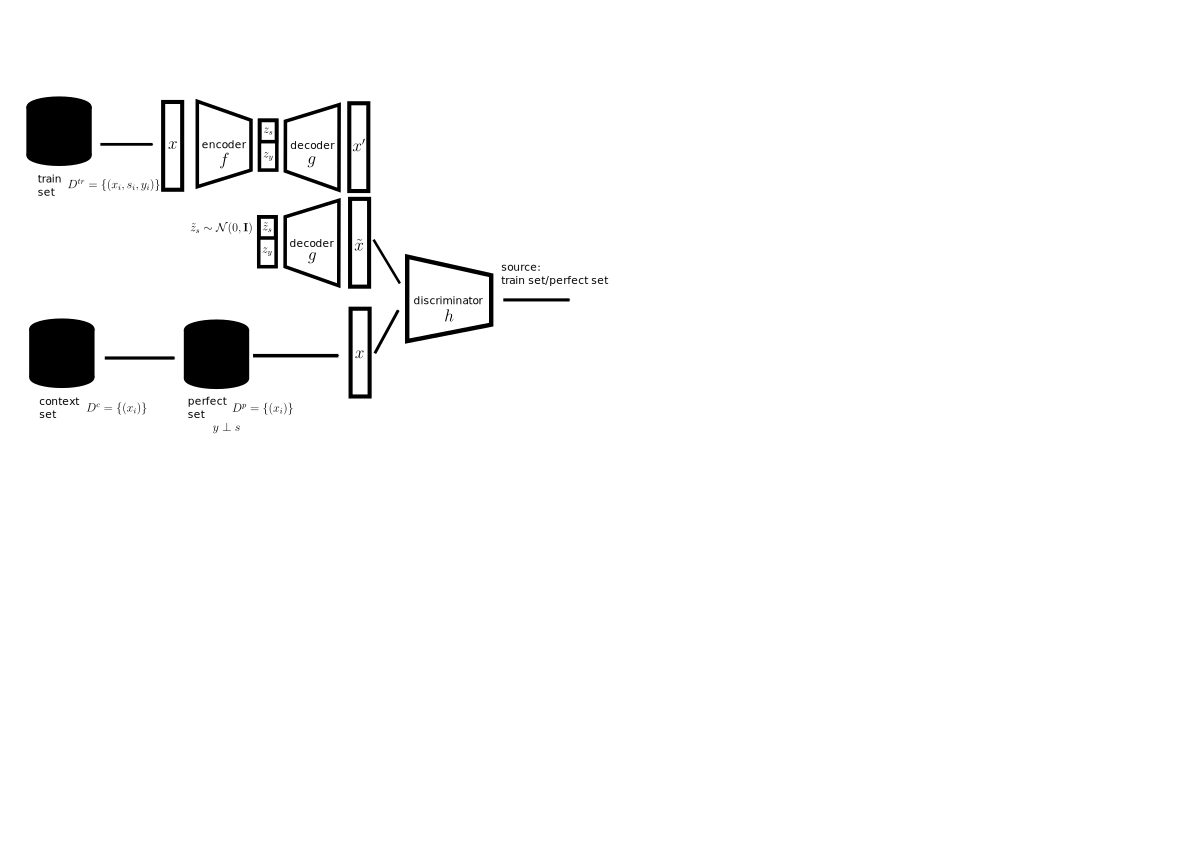
\includegraphics[width=0.9\textwidth]{supmatch/figures/SSL-framework}
    % 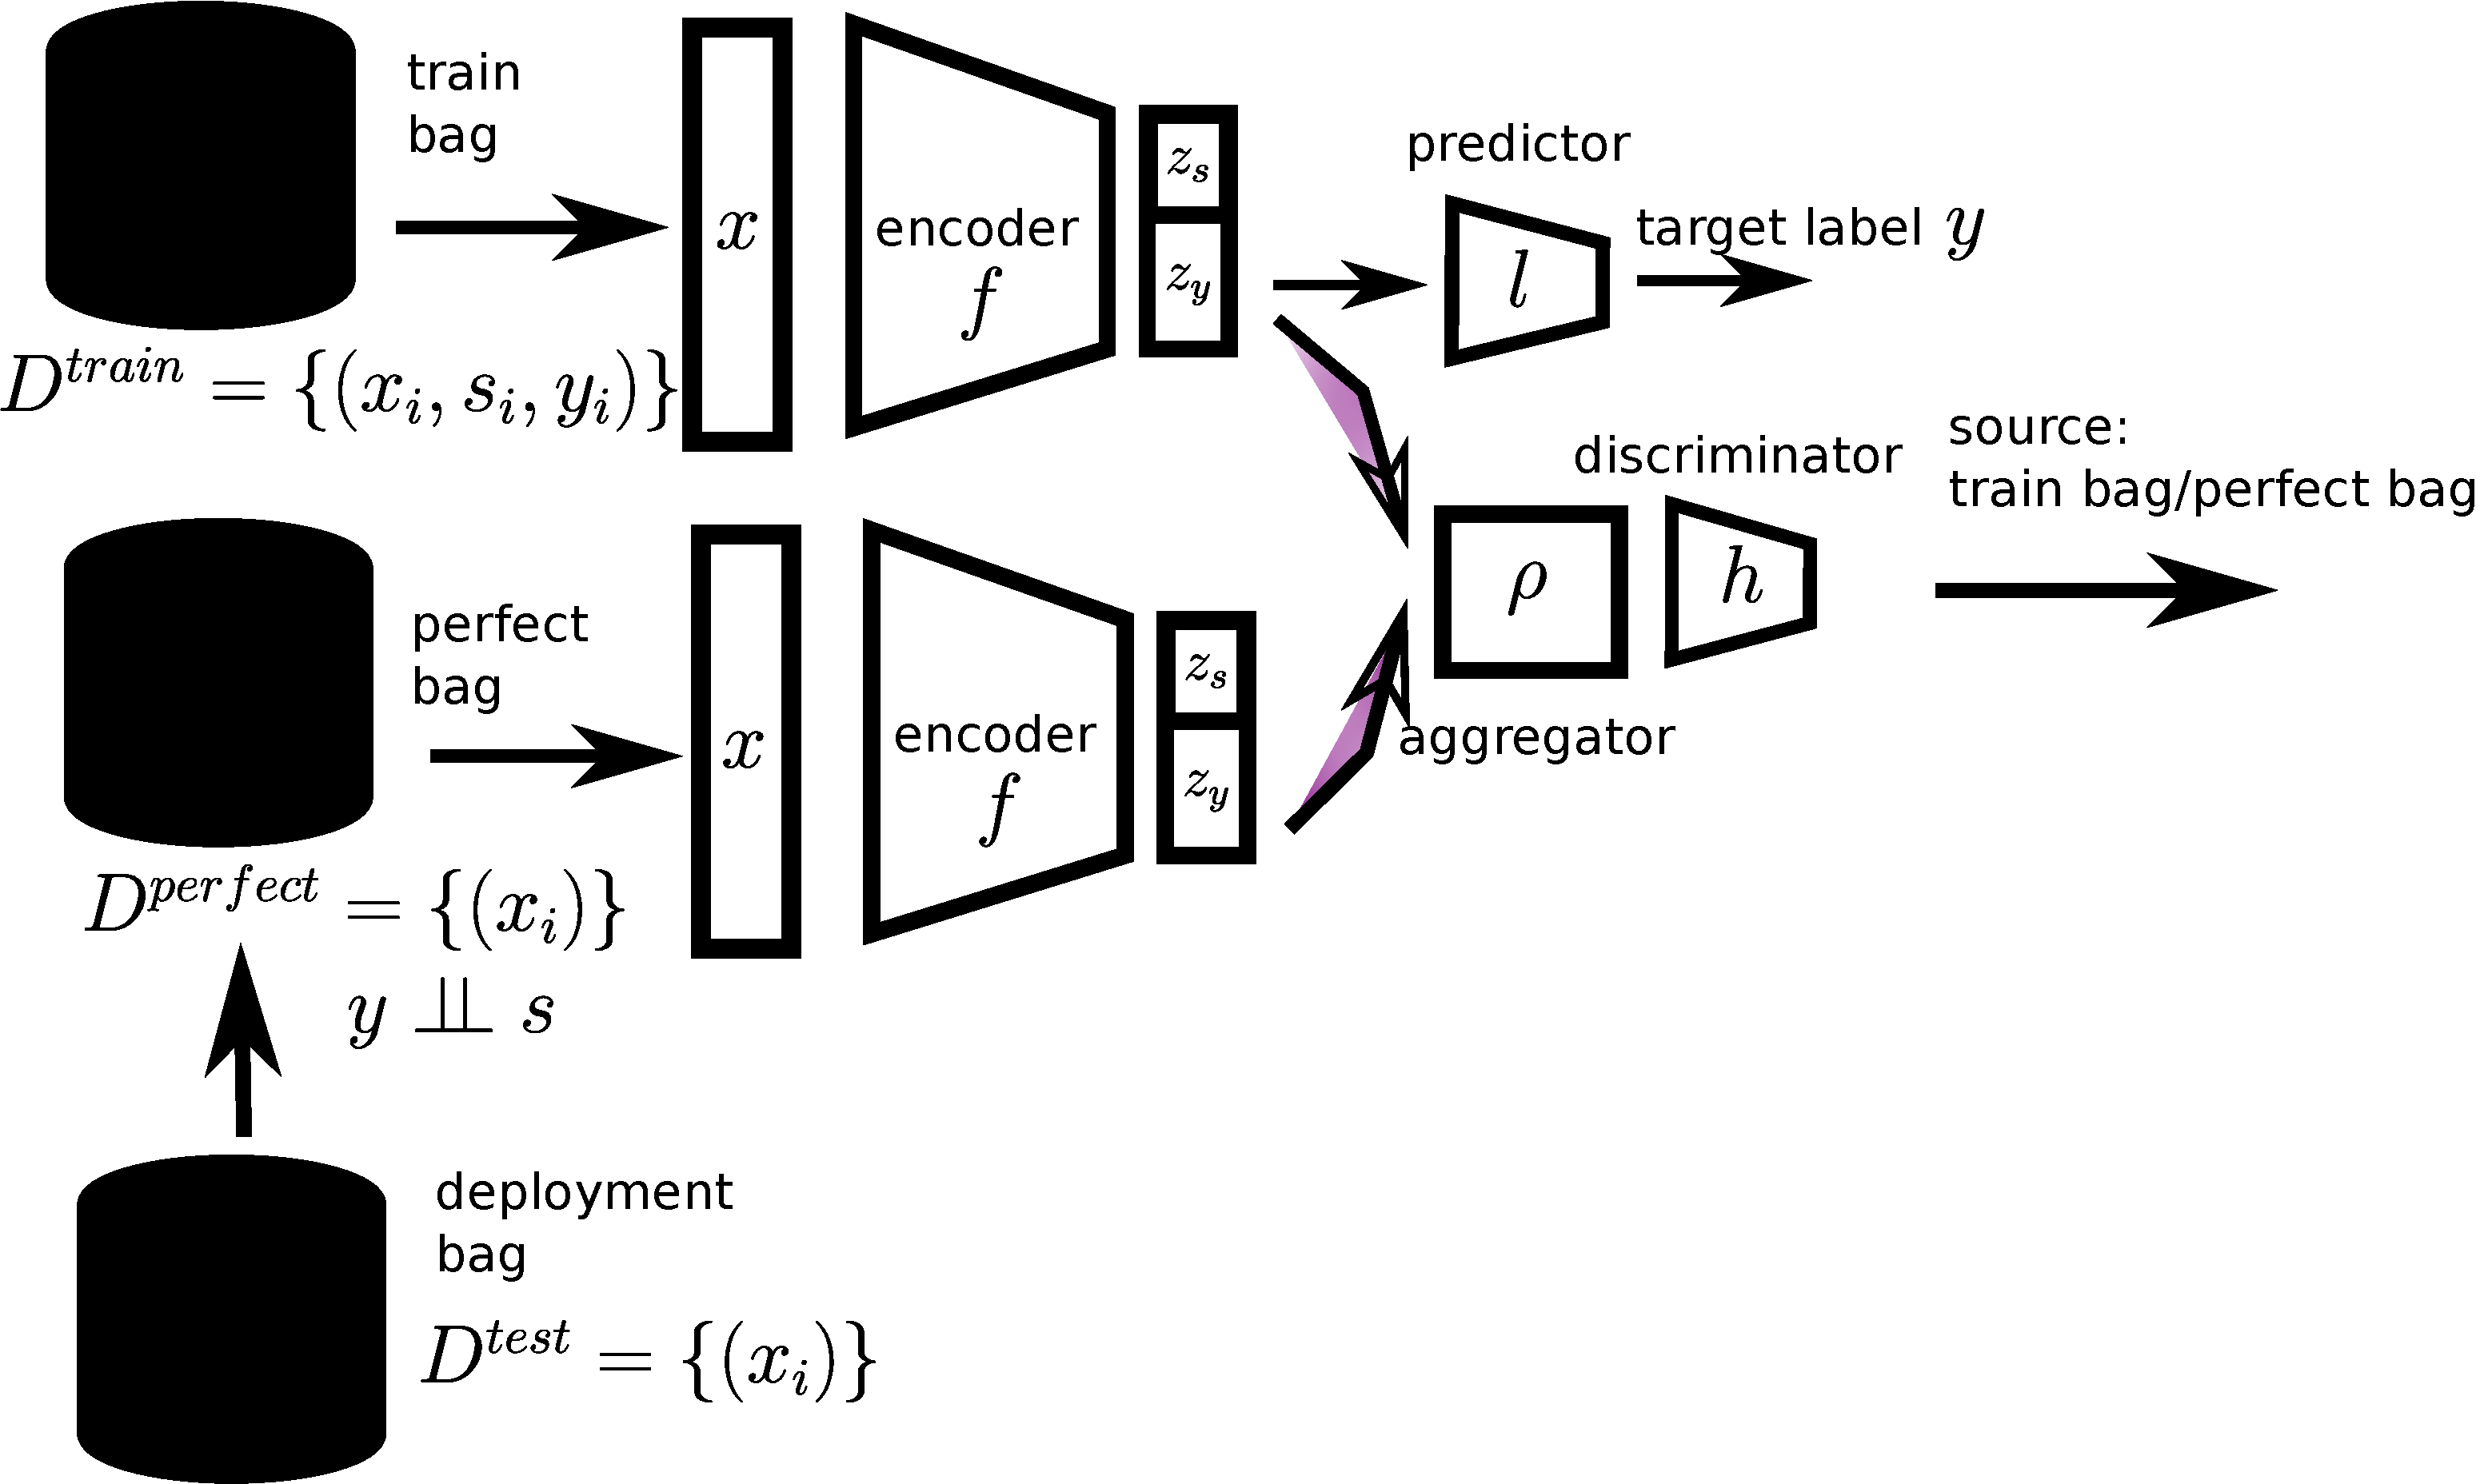
\includegraphics[width=\textwidth]{supmatch/figures/SSL-framework-withPred.pdf}
    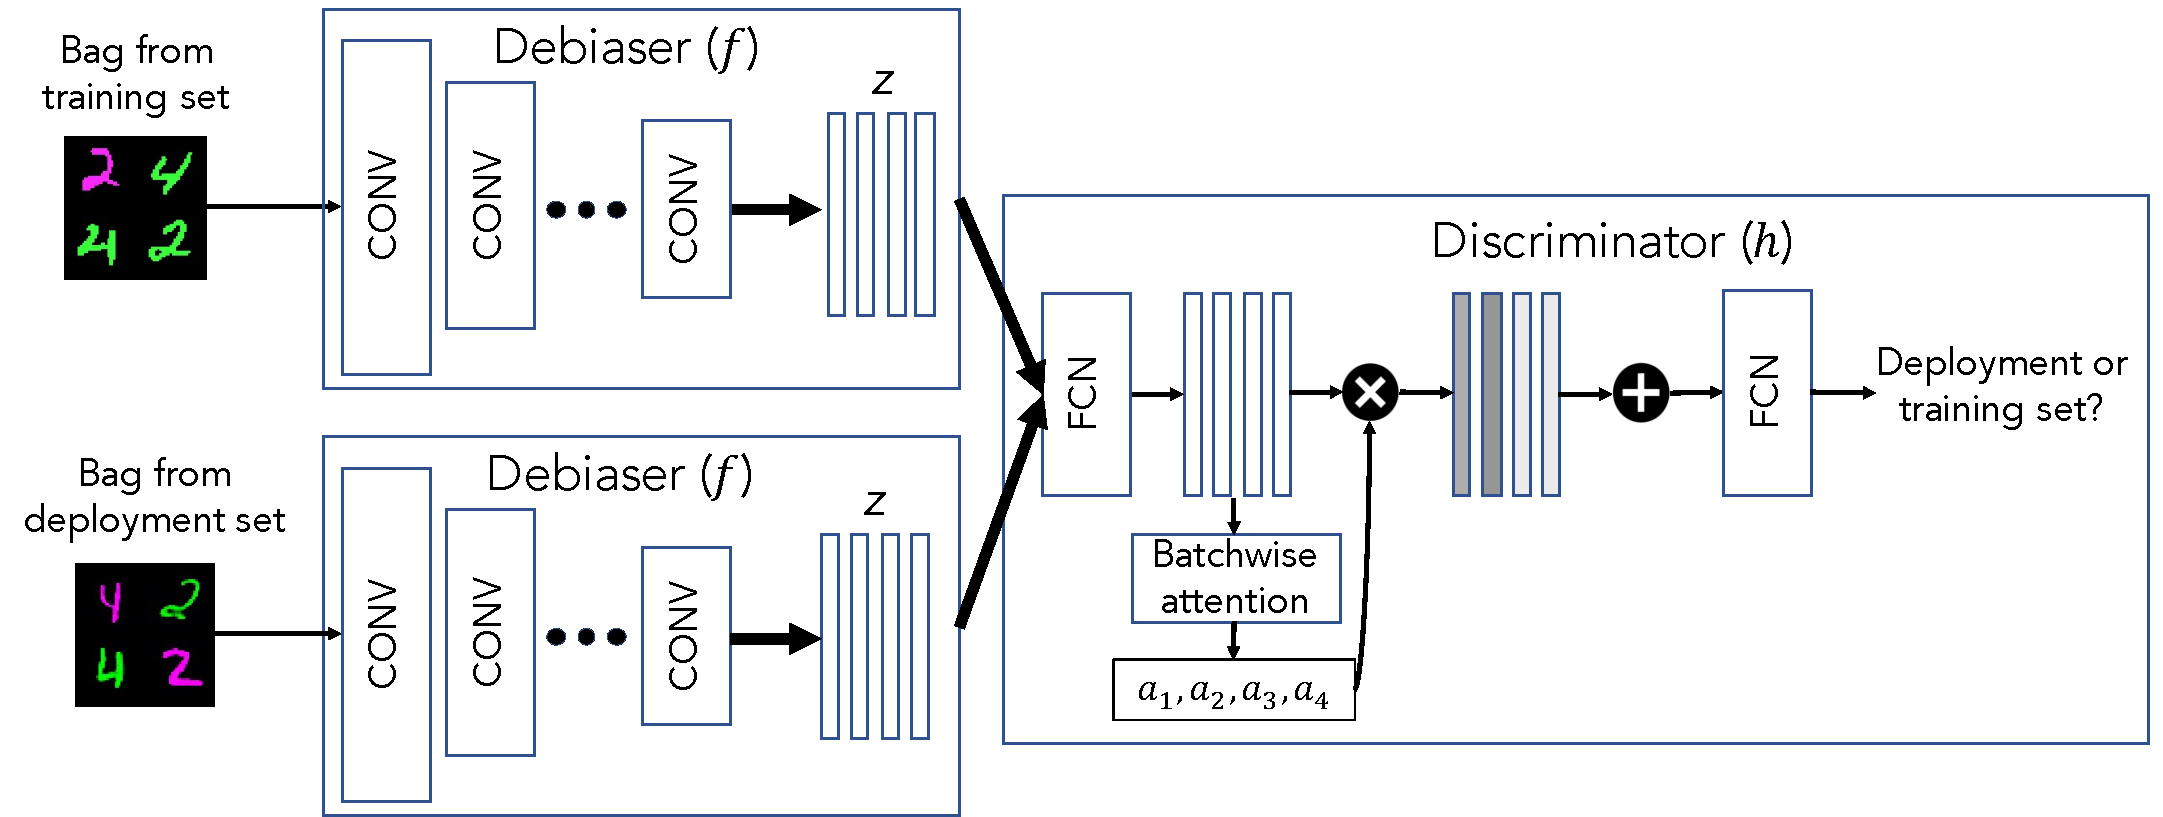
\includegraphics[width=\textwidth]{supmatch/figures/illustrations/architecture.pdf}
    \caption{% The main components of our support-matching algorithm, $f$ (debiaser) and $h$
      (discriminator). The debiaser is trained to produce encodings, $z$ of the data that are
      invariant to the subgroups differences. %source dataset and thereby the subgroups identifying
      it. In order to determine whether a bag of encodings originates from the training set or the
      deployment set, the discriminator performs an attention-weighted aggregation over the bag
      dimension to model interdependencies between the samples. In the case of Coloured MNIST where
      {\color{purple}purple} fours constitute the missing subgroup, the discriminator can identify
      an encoding of a bag from the training set by the absence of such samples as long as color
      information is detectable in $z$. %, thereby serving as an error signal for the debiaser. By
    learning a subgroup invariant representation, the debiaser can hide the origin of the bags from
  the discriminator.} \label{fig:architecture}
\end{figure*}%
%
We give a more detailed explanation of the model used in our method.
Fig.~\ref{fig:architecture} shows the core of our method:
the debiaser, $f$, which produces bags of encodings, $z$
-- on both the training and the deployment set --
which are then fed to a discriminator that tries to identify the origin of the bags.
The discriminator uses batch-wise attention in order to consider a bag as a whole,
which allows cross-comparisons.
%
\subsection{Details of the attention mechanism}\label{ssec:attention-mechanism}
%
The \emph{discriminator} function $h$ that predicts which dataset a bag of samples embedded in $z$
was sampled from should have the following property: \( h((f(x) | x \in B)) = h((f(x) | x \in \pi
(B))) \) for all permutations $\pi$, and $f: x \to z$. 
%
For the entirety of function $h$ -- composed of sub-functions \( h_1(h_2(h_3...))) \) -- to have this
property, it suffices that only the innermost sub-function, $\rho$, does. 
%
While there are a number of choices when it comes to defining $\rho$, we choose a weighted average
$\rho = \frac{1}{|\mathcal{B}|} \sum_{x \in B}\mathrm{attention}(f(x), B) \cdot f(x)$, with weights
computed according to a learned attention mechanism. 
%
The idea of using an attention mechanism for set-wise classification has been previously explored
to great success by, e.g.\ \citet{lee2019set}. %\cite{ilse2018attention} and \cite{lee2019set}. 
%
We employ an bag-wise attention mechanism based on the scaled dot-product attention of
\citet{vaswani2017attention}, where in our case we define $K$ and $V$ to be linear projections of
$z$ -- $zW_k$ and $zW_v$, respectively -- and $Q$ to be mean of another linear projection of $z$,
$zW_q$, taken over the bag dimension.

\begin{align*}
  \text{Attention}(\mathit{Q}, \mathit{K}, \mathit{V}) := \text{Softmax} \biggl( \frac{ \mathit{Q}
  \mathit{K}^T  } { \sqrt{d} } \biggr) V
\end{align*}

The output of $\rho$ is then further processed by a series of fully-connected layers and the final
output is the binary prediction for a given bag of samples.

\subsection{Training procedure and hyperparameters}
\begin{table*}[tp]
 \centering
 \caption{Selected hyperparameters for experiments with Coloured MNIST, Adult and CelebA datasets.}
 \label{tab:hparams}
 \scalebox{0.8}{
 \begin{tabular}{llll}
 \toprule
 & \textbf{Coloured MNIST} & \textbf{Adult} & \textbf{CelebA}       
 \\ & 2-dig SB / 2-dig MS / 3-dig SB
 \\ \midrule
 Input size  &   $3 \times 32 \times 32$ & $61$ & $3 \times 64 \times 64$ \\  \midrule
 \multicolumn{4}{c}{AutoEncoder}                     \\ \midrule
 Levels                      & $4$         & $1$    & $5$\\
 Level depth                 & $2$         & $1$    & $2$\\
 Hidden units / level        & $[32, 64, 128, 256]$ & $[61]$ & $[32, 64, 128, 256, 512]$\\
 Activation                  & GELU        & GELU   & SiLU  \\
 Layer-wise Normalisation               & -           & -      & LayerNorm \\
 Downsampling op.  & Strided Convs. & -- & Strided Convs.\\
 Reconstruction loss         & MSE         & Mixed$^1$  & MSE \\
 Learning rate               & $1 \times 10^{-3}$   & $1 \times 10^{-3}$  & $1 \times 10^{-3}$ \\ \midrule
 \multicolumn{4}{c}{Clustering}                      \\ \midrule
 Batch size                  & $256$      & $1000$  & $256$ \\
 AE pre-training epochs      & $150$        & $100$ & $10$  \\
 Clustering epochs           & $100$       & $300$  & $20$ \\
 Self-supervised loss & Cosine + BCE & Cosine + BCE & Cosine \\
 U (for ranking statistics)             & $5$         & $3$     & $8$    \\   \midrule
 \multicolumn{4}{c}{Support-Matching}                   \\ \midrule
 Batch size & $1$/$32$/$14$  & $64$   & $32$ \\
 Bag size   & $256$/$8$/$18$ & $32$ & $8$ \\
 Training iterations    & $8\text{k}/8\text{k}/20\text{k}$ & $5\text{k}$ & $2\text{k}$ \\
 Encoding ($z$) size$^2$  & $128$   & $35$  & $128$ \\
 Binarised $\tilde{s}$ & \xmark\, / \cmark\, / \cmark & \xmark & \xmark \\
 $y$-predictor weight ($\lambda_1$) & $1$ & $0$ & $1$  \\ 
 $s$-predictor weight ($\lambda_2$) & $1$ & $0$ & $1$  \\ 
 Adversarial weight ($\lambda_3$)   & $1 \times
 10^{-3}$   & $1$   & $1$\\ 
 Stop-gradient $\left(\nabla_\theta h_\psi(f_\theta(X^\mathit{dep}))=0\right)$ & \xmark & \cmark & \xmark \\
 \midrule
 \multicolumn{4}{c}{Predictors}   \\ \midrule
 Learning rate  & $3 \times 10^{-4}$ &   $1 \times 10^{-3}$  $ 1 \times 10^{-3}$\\
 \midrule
 \multicolumn{4}{c}{Discriminator}                   \\ \midrule
 Attention mechanism$^3$    & Gated   & Gated & Gated \\
 Hidden units pre-aggregation  & $[256, 256]$  & $[32]$ & $[256, 256]$\\
 Hidden units post-aggregation & $[256, 256]$ & --  & $[256, 256]$ \\
 Embedding dim (for attention) & $32$ & $128$ & $128$ \\
 Activation & GELU & GELU & GELU \\
 Learning rate  & $3 \times 10^{-4}$    & $1 \times 10^{-3}$ & $1 \times 10^{-3}$\\
 Updates / AE update    & $1$  & $3$    & $1$    \\
 \bottomrule
 \addlinespace
 \multicolumn{4}{p{17cm}}{\footnotesize $^1$ Cross-entropy is used for categorical features, MSE for continuous features.} \\
 \multicolumn{4}{p{17cm}}{\footnotesize $^2$ $|z|$ denotes the combined size of $\tilde{s}$ and
 $z$, with the former occupying $\ceil{\text{log}_2(\gS)}$ dimensions, the latter the remaining dimensions.} \\
 \multicolumn{4}{p{17cm}}{
 \footnotesize $^3$ 
 The attention mechanism used for computing the sample-weights within a bag. \emph{Gated} refers to
 gated attention  proposed by \citet{ilse2018attention}, while \emph{SDP} refers to the scaled
 dot-product attention proposed by \citet{vaswani2017attention}.
 }
 \end{tabular}
 }
 % add empty lines to make the table take up a full page
 ~\\
 ~\\
 ~\\
\end{table*}

The hyperparameters and architectures for the \acf{AE} (\texttt{AE}), Predictor and Discriminator
sub-networks are detailed in Table \ref{tab:hparams} for all three datasets.We train all models
using \texttt{Adam} \citep{KinBa15}.

For the Coloured MNIST and CelebA datasets, the baseline \texttt{ERM}, \texttt{DRO}, \texttt{LfF}
(in the case of the former) and \texttt{gDRO} (in the case of the latter) models use a
convolutional backbone consisting of one Conv-BN-LReLU block per ''stage``, with each stage
followed by max-pooling operation to spatially downsample by a factor of two to produce the
subsequent stage. This backbone consists of 4 and 5 stages for Coloured MNIST and CelebA,
respectively. The output of the backbone is flattened and fed to a  single fully-connected layer of
size $|Y|$ in order to obtain the class-prediction, $\hat{y_i}$, for a given instance. To evaluate
our method, we simply train a linear classifier on top of $z$; this is sufficient due to
linear-separability being encouraged during training by the $y$-predictor. For the Adult Income
dataset, we use an \ac{MLP} composed of a single hidden layer 35 units in size, followed by a SELU
activation \citep{klambauer2017self}, as both the downstream classifier for our method, and as the
network architecture of the baselines. All baselines and downstream classifiers alike were trained
for $60$ epochs with a learning rate of $1 \times 10^{-3}$ and a batch size of $256$.

Since, by design, we do not have labels for all subgroups the model will be tested on, and bias
against these missing subgroups is what we aim to combat, properly validating, and thus conducting
hyperparameter selection for models generally, is not straightforward. Indeed, performing
model-selection for domain generalisation problems is well-known to be a difficult problem
\citep{gulrajani2021search}. We can use estimates of the mutual information between the
learned-representation and $s$ and $y$ (which we wish to minimize \wrt{} to the former, maximise
\wrt{} the latter) to guide the process, though optimizing the model w.r.t.\ to these metrics
obtained from only the training set does not guarantee generalisation to the missing subgroups. We
can, however, additionally measure the entropy of the predictions on the encoded test set and seek
to maximise it across all samples, or alternatively train a discriminator of the same kind used for
distribution matching as a measure of the shift in the latent space between datasets. We use the
latter approach (considering the combination of the learned distance between subspace distributions
and reconstruction loss) to inform an extensive grid-search over the hyperparameter space for our
method.

For the \texttt{DRO} baseline, we allowed access to the labels of the test set for the purpose of
hyperparameter selection, performing a grid-search over multiple splits to avoid overfitting to any
particular instantiation. Specifically, the threshold ($\eta$) parameter for \texttt{DRO} was
determined by a grid-search over the space $\{0.01, 0.1, 0.3, 1.0\}$.

% In addition to the losses stated in the support-matching objective, $\mathcal{L}$, in the main
% text, we also regularize the encoder by the $\ell^2$ norm of its embedding, multiplied by a small
% pre-factor, finding this to work better than more complex regularization methods, such as spectral
% normalization \cite{miyato2018spectral}, for stabilizing adversarial training. \section{Additional
% analysis of results}\label{sec:additional-analysis}

\subsection{Visualisations of results}\label{sec:qual-results}
\begin{figure}[tp]
  \centering
  \begin{subfigure}[b]{0.49\columnwidth}
    \centering
    % 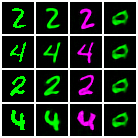
\includegraphics[width=\textwidth]{supmatch/example_images/fresh-dawn-2179_train_reconstructions_9900.png}
    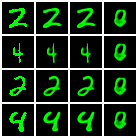
\includegraphics[width=\textwidth]{supmatch/example_images/copper-microwave-2174_train_reconstructions_9900.png}
    \caption{
    Different reconstructions on the training set. Corresponding to: original, full reconstruction,
    reconstruction of $z$ ($\tilde{s}$ zeroed out), reconstruction of $\tilde{s}$ ($z$ zeroed out).
    }%
    \label{fig:cmnist-recon-training}
  \end{subfigure}
   \hfill
%   \quad
  \begin{subfigure}[b]{0.49\columnwidth}
    \centering
    % 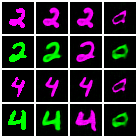
\includegraphics[width=\textwidth]{supmatch/example_images/fresh-dawn-2179_context_reconstructions_9900.png}
    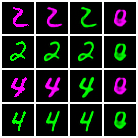
\includegraphics[width=\textwidth]{supmatch/example_images/copper-microwave-2174_context_reconstructions_9900.png}
    \caption{
    Different reconstructions on the deployment set. Corresponding to: original, full
    reconstruction, reconstruction of $z$ ($\tilde{s}$ zeroed out), reconstruction of $\tilde{s}$
    ($z$ zeroed out).
    }%
    \label{fig:cmnist-recon-deployment}
  \end{subfigure}
  \caption{
   Visualisation of our method's solutions for the Coloured MNIST dataset, with
   {\color{purple}purple} as the missing subgroup. In each of the subfigures
   \ref{fig:cmnist-recon-training} and \ref{fig:cmnist-recon-deployment}: Column 1 shows the
   original images from $x$ from the respective set. Column 2 shows plain reconstructions generated
   from $x_\textit{recon}=g(f(x), t(x))$. Column 3 shows reconstruction with zeroed-out
   $\tilde{s}$: $g(f(x), 0)$, which effectively visualizes $z$. Column 4 shows the result of an
   analogous process where $z$ was zeroed out instead.
  }%
  \label{fig:cmnist-recon}
\end{figure}%
%
\begin{figure}[tp]
  \centering
  \begin{subfigure}[b]{0.49\columnwidth}
    \centering
    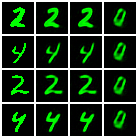
\includegraphics[width=\textwidth]{supmatch/example_images/zany-glade-2191_train_reconstructions_9900.png}
    \caption{
    Different reconstructions on the training set. Corresponding to: original, full reconstruction,
    reconstruction of $z$ ($\tilde{s}$ zeroed out), reconstruction of $\tilde{s}$ ($z$ zeroed out).
    }%
    \label{fig:cmnist-recon-training-failure}
  \end{subfigure}
   \hfill
%   \quad
  \begin{subfigure}[b]{0.49\columnwidth}
    \centering
    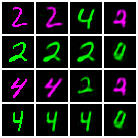
\includegraphics[width=\textwidth]{supmatch/example_images/zany-glade-2191_context_reconstructions_9900.png}
    \caption{
    Different reconstructions on the deployment set. 
    %
    Corresponding to: original, full reconstruction, reconstruction of $z$ ($\tilde{s}$ zeroed
    out), reconstruction of $\tilde{s}$ ($z$ zeroed out).
    }%
    \label{fig:cmnist-recon-deployment-failure}
  \end{subfigure}
  \caption{
    %
   Visualisation of a failure of our method for the Coloured MNIST dataset, with
   {\color{purple}purple} as the missing subgroup. 
   %
   In each of the subfigures \ref{fig:cmnist-recon-training-failure} and
   \ref{fig:cmnist-recon-deployment-failure}: Column 1 shows the original images from $x$ from the
   respective set. Column 2 shows plain reconstructions generated from $x_\textit{recon}=g(f(x),
   t(x))$. Column 3 shows reconstruction with zeroed-out $\tilde{s}$: $g(f(x), 0)$, which
   effectively visualises $z$. Column 4 shows the result of an analogous process where $z$ was
   zeroed out instead.
   %
  }%
  \label{fig:cmnist-recon-failure}
\end{figure}%
%
\begin{figure}[htp]
     \centering
     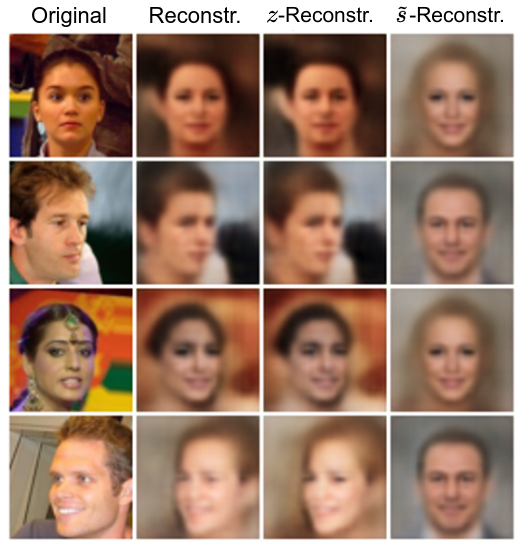
\includegraphics[width=0.5\textwidth]{supmatch/example_images/reconstructions_celeba.png}
     \caption{%
       %
       Visualisation of our method's solutions for the CelebA dataset, with ``smiling females'' as
       the missing subgroup. 
     %
       Column 1 shows the original images from $x$ from the deployment set of CelebA. 
     %
       Column 2 shows plain reconstructions generated from $x_\textit{recon}=g(f(x), t(x))$.
     %
       Column 3 shows reconstruction with zeroed-out $\tilde{s}$: $g(f(x), 0)$, which effectively
       visualises $z$. 
     %
       Column 4 shows the result of an analogous process where $z$ was zeroed out instead.
     %
     }%
     \label{fig:celeba-recons}
\end{figure}%
%
\begin{figure*}[htp]
  \centering
    \begin{subfigure}[b]{0.49\textwidth}
    
\includegraphics[width=\textwidth]{supmatch/figures/celeba_attn_map.png}
    \end{subfigure}
    \hfill
    \begin{subfigure}[b]{0.49\textwidth}
    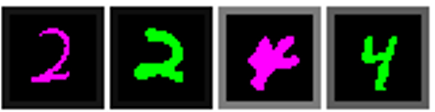
\includegraphics[width=\textwidth]{supmatch/figures/cmnist_attn_map.png}
    \end{subfigure}
  \caption{
    Example sample-wise attention maps for bags of CelebA (left) and CMNIST (right) images sampled
    from a balanced deployment set. 
    %
    The training set is biased according to the \emph{subgroup bias} setting where for CelebA
    ``smiling females'' constitute the missing source and for Coloured MNIST {\color{purple}purple}
    fours constitute the missing source. 
    %
    The attention weights are used during the discriminator's aggregation step to compute a
    weighted sum over the bag. 
    %
    The attention-weight assigned to each sample is proportional to the lightness of its frame,
    with black signifying a weight of 0, white a weight of 1. 
    %
    Those samples belonging to the missing subgroup are assigned the highest weight as they signal
    from which dataset (training vs.\ deployment) the bag containing them was drawn from. 
%
}
  \label{fig:attn_maps}
\end{figure*}%
%
We show qualitative results of the disentangling in figures \ref{fig:cmnist-recon},
\ref{fig:cmnist-recon-failure} (both Coloured MNIST), and \ref{fig:celeba-recons} (CelebA).
Fig.~\ref{fig:cmnist-recon} shows successful disentangling (from a run that achieved close to 100\%
accuracy); in the deployment set the representation $z$ has lost all colouring (see column 3 in the
figures). 
%
Fig.~\ref{fig:cmnist-recon-failure} on the other hand, shows a visualisation from a \emph{failed}
run; instead of encoding purple 2's and green 2's with the same representation, the model here
encoded purple 2's and green 4's as similar. 
%
This is a valid solution of the given optimisation problem -- the representation is invariant to
training set vs deployment set -- but it is definitely not the intended solution.

Fig.~\ref{fig:celeba-recons} shows visualisations for CelebA. 
%
With a successful disentangling, column 3 (visualisation of $z$) should show a version of the image
that is ``gender-neutral'' (i.e.\ invariant to gender). 
%
Furthermore, column 4 (visualisation of $\tilde{s}$) should be invariant to the class label (i.e.\
``smiling''), so the images should either be all with smiles or all without smiles.

Fig.~\ref{fig:attn_maps} shows attention maps for bags from the deployment set. 
%
We can see that the model pays special attention to those samples that are not included in the
training set. For details, see the captions.

\subsection{Additional metrics}\label{sec:additional-metrics}
%
Figures~\ref{fig:cmnist-2v4-partial-add}, \ref{fig:cmnist-2v4-miss-s-add},  and
\ref{fig:celeba-gender-smiling-add} show the \ac{TPR} ratio and the \ac{TNR} ratio as additional
metrics for Coloured MNIST (2 digits) and CelebA. 
%
These are computed as the ratio of \ac{TPR} (or \ac{TNR}) on subgroup $s=0$ over the \ac{TPR} (or
\ac{TNR}) on subgroup $s=1$; if this gives a number greater than 1, the inverse is taken. 
%
Similarly to the PR ratio reported in the main paper, these ratios give an indication of how much
the prediction of the classifier depends on the subgroup label $s$.

Fig.~\ref{fig:cmnist-3dig-4miss-add} shows metrics specific to multivariate $s$ (i.e.\ non-binary
$s$). 
%
We report the minimum (i.e.\ farthest away from \(1\) of the pairwise ratios (\ac{TPR}/\ac{TNR}
ratio min) as well as the largest difference between the raw values (\ac{TPR}/\ac{TNR} diff max). 
%
Additionally, we compute the \ac{HGRMC} between $S$ and $Y$, serving as a measure of dependence
defined between two variables with arbitrary support.
%
\begin{figure*}[htp]
  \centering
%   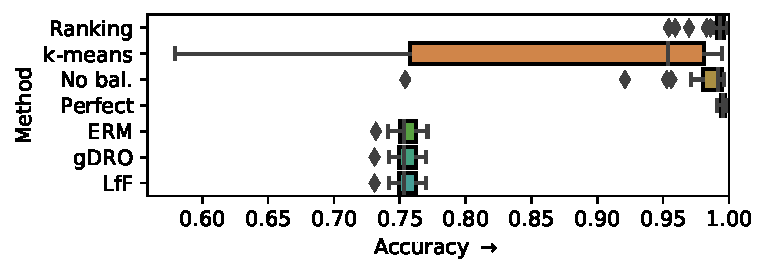
\includegraphics[width=\columnwidth]{supmatch/figures/cmnist_2v4_partial_acc.pdf}
%   \includegraphics[width=\columnwidth]{supmatch/figures/cmnist_2v4_partial_pr.pdf}
%   \includegraphics[width=\columnwidth]{supmatch/figures/cmnist_2v4_partial_tpr.pdf}
%   \includegraphics[width=\columnwidth]{supmatch/figures/cmnist_2v4_partial_tnr.pdf}
  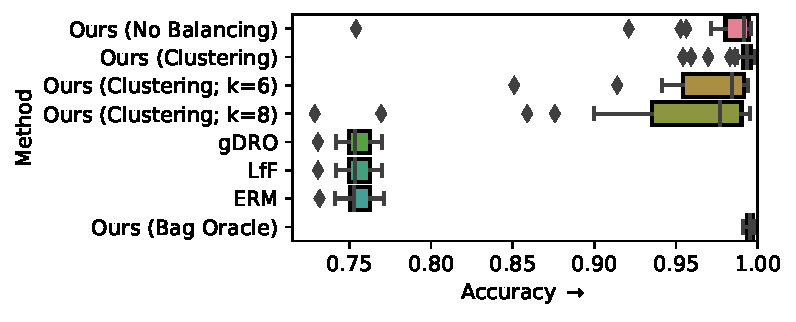
\includegraphics[width=0.49\textwidth]{supmatch/figures/cmnist/subgroup_bias_oc/cmnist_2v4_partial_overcluster_acc.pdf}
  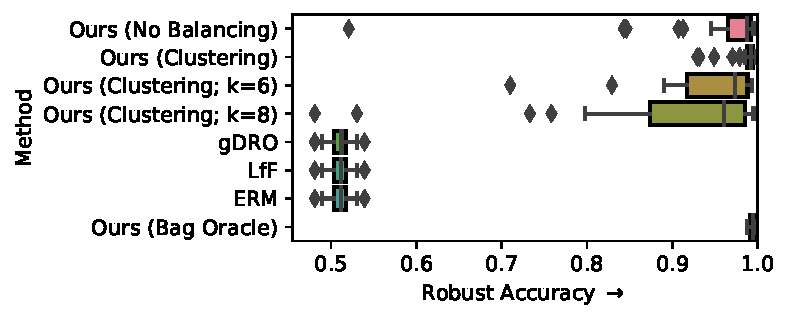
\includegraphics[width=0.49\textwidth]{supmatch/figures/cmnist/subgroup_bias_oc/cmnist_2v4_partial_overcluster_acc-min.pdf}
  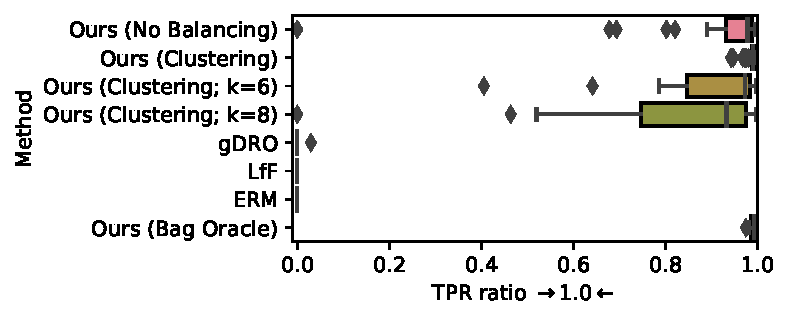
\includegraphics[width=0.49\textwidth]{supmatch/figures/cmnist/subgroup_bias_oc/cmnist_2v4_partial_overcluster_tprr.pdf}
    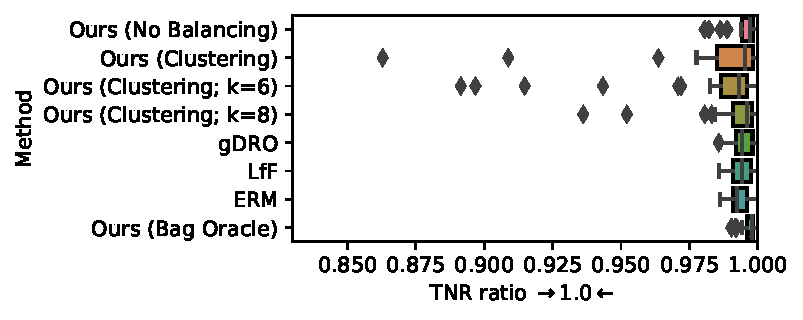
\includegraphics[width=0.49\textwidth]{supmatch/figures/cmnist/subgroup_bias_oc/cmnist_2v4_partial_overcluster_tnrr.pdf}
  \caption{
    Results from \textbf{30 repeats} for the Coloured MNIST dataset with two digits, 2 and 4, with
    \emph{subgroup bias} for the colour `{\color{purple}purple}': for {\color{purple}purple}, only
    the digit class `2' is present.
    \textbf{Top left}: Accuracy.
    \textbf{Top right}: Positive rate ratio.
    \textbf{Bottom left}: True positive rate ratio.
    \textbf{Bottom right}: True negative rate ratio.
    For \texttt{Ours (Clustering)}, the clustering accuracy was 96\% $\pm$ 6\%.
    % for \texttt{K-means} it was 64\% $\pm$ 10\%.
    For an explanation of \texttt{Ours (Clustering; k=6/8)} see \S\ref{sec:sm-overclustering}.
  }%
  \label{fig:cmnist-2v4-partial-add}
\end{figure*}
\begin{figure*}[htp]
  \centering
  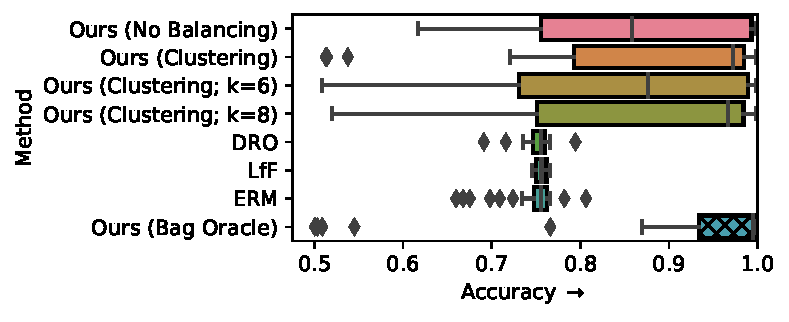
\includegraphics[width=0.49\textwidth]{supmatch/figures/cmnist/missing_subgroup_oc/cmnist_2v4_miss_s_overcluster_acc.pdf}
  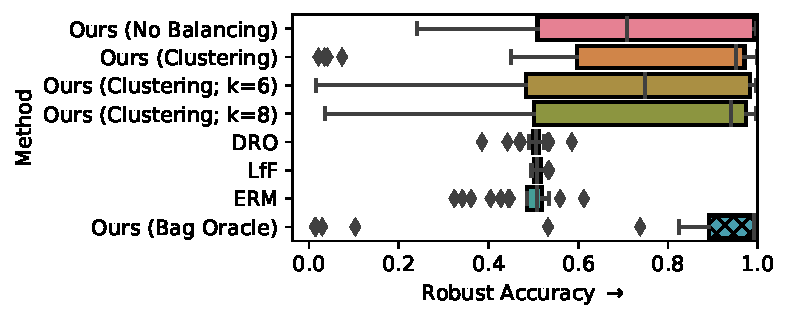
\includegraphics[width=0.49\textwidth]{supmatch/figures/cmnist/missing_subgroup_oc/cmnist_2v4_miss_s_overcluster_acc-min.pdf}
  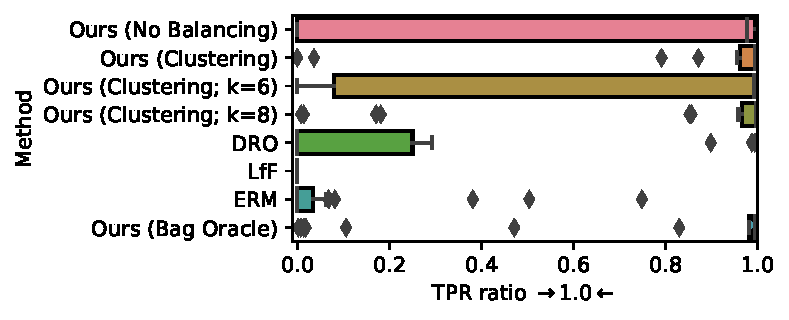
\includegraphics[width=0.49\textwidth]{supmatch/figures/cmnist/missing_subgroup_oc/cmnist_2v4_miss_s_overcluster_tprr.pdf}
  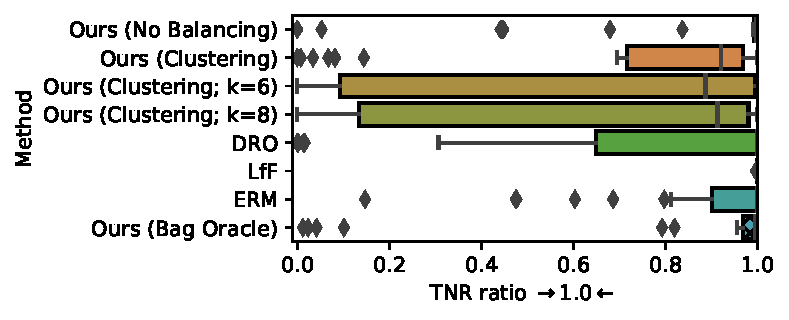
\includegraphics[width=0.49\textwidth]{supmatch/figures/cmnist/missing_subgroup_oc/cmnist_2v4_miss_s_overcluster_tnrr.pdf}

  \caption{
    Results from \textbf{30 repeats} for the Coloured MNIST dataset with two digits, 2 and 4, with a
    \emph{missing subgroup}: the training dataset only has {\color{green}green} digits.
    \textbf{Top left}: Accuracy.
    \textbf{Top right}: Robust Accuracy.
    \textbf{Bottom left}: True positive rate ratio.
    \textbf{Bottom right}: True negative rate ratio.
    For \texttt{Ours (Clustering)}, the clustering accuracy was 88\% $\pm$ 5\%.
    % for \texttt{K-means} it was 72\% $\pm$ 16\%.
    For an explanation of \texttt{Ours (Clustering; k=6/8)} see \S\ref{sec:sm-overclustering}.
  }%
  \label{fig:cmnist-2v4-miss-s-add}
\end{figure*}

\begin{figure*}[htp]
  \centering
  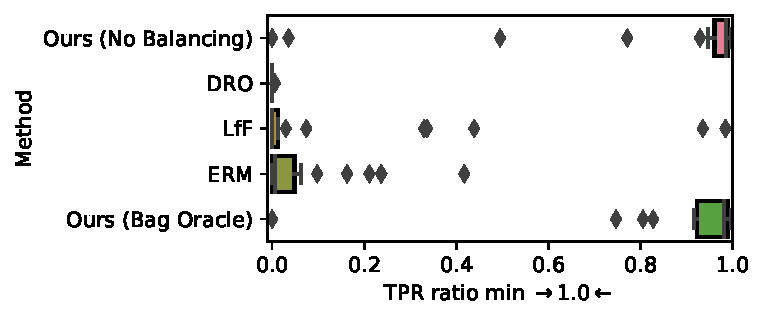
\includegraphics[width=0.49\textwidth]{supmatch/figures/cmnist/supmat/cmnist_3dig_4miss_tprr-min.pdf}
  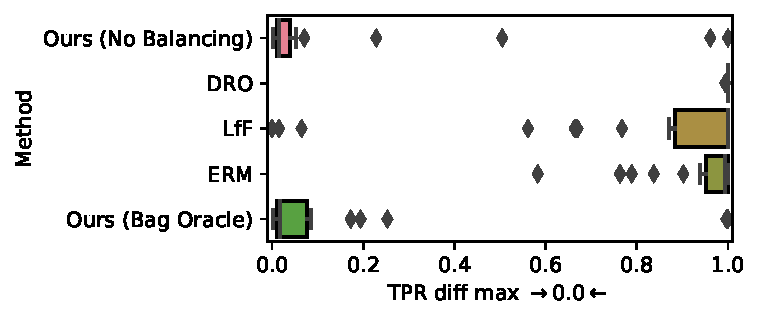
\includegraphics[width=0.49\textwidth]{supmatch/figures/cmnist/supmat/cmnist_3dig_4miss_tprd-max.pdf}
  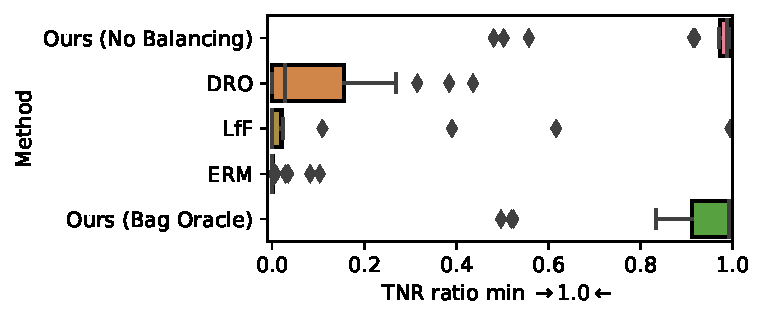
\includegraphics[width=0.49\textwidth]{supmatch/figures/cmnist/supmat/cmnist_3dig_4miss_tnrr-min.pdf}
  \includegraphics[width=0.49\textwidth]{supmatch/figures/cmnist/supmat/cmnist_3dig_4miss_tnrd-max.pdf}
  \caption{
    Results from \textbf{30 repeats} for the Coloured MNIST dataset with three digits: `2', `4' and
    `6'. Four combinations of digit and color are missing: {\color{green}green} 2's,
    {\color{blue}blue} 2's, {\color{blue}blue} 4's and {\color{green}green} 6's.
    % \textbf{First row}: Hirschfeld-Gebelein-R\'enyi maximal correlation between $S$ and $Y$.
    % \textbf{First row, left}: minimum of all positive rate ratios.
    % \textbf{First row, right}: maximum of all positive rate differences.
    \textbf{First row, left}: minimum of all true positive rate ratios.
    \textbf{First row, right}: maximum of all true positive rate differences.
    \textbf{Second row, left}: minimum of all true negative rate ratios.
    \textbf{Second row, right}: maximum of all true negative rate differences.
  }%
  \label{fig:cmnist-3dig-4miss-add}
\end{figure*}
  
\begin{figure*}[t]
  \centering
  % Smiling females missing
%   \normalsize{Missing source: smiling females}\par\medskip
 \includegraphics[width=0.49\textwidth]{supmatch/figures/celeba/no_smiling_females/celeba_gender_smiling_tprr.pdf}
 \includegraphics[width=0.49\textwidth]{supmatch/figures/celeba/no_smiling_females/celeba_gender_smiling_tnrr.pdf}
    % Smiling males missing
%   \normalsize{Missing source: smiling males}\par\medskip
 \includegraphics[width=0.49\textwidth]{supmatch/figures/celeba/no_smiling_males/celeba_gender_smiling_tprr.pdf}
 \includegraphics[width=0.49\textwidth]{supmatch/figures/celeba/no_smiling_males/celeba_gender_smiling_tnrr.pdf}
    % Unsmiling females missing
%   \normalsize{Missing source: non-smiling} females\par\medskip
 \includegraphics[width=0.49\textwidth]{supmatch/figures/celeba/no_unsmiling_females/celeba_gender_smiling_tprr.pdf}
 \includegraphics[width=0.49\textwidth]{supmatch/figures/celeba/no_unsmiling_females/celeba_gender_smiling_tnrr.pdf}
  % Unsmiling males missing
%   \normalsize{Missing source: non-smiling males}\par\medskip
 \includegraphics[width=0.49\textwidth]{supmatch/figures/celeba/no_unsmiling_males/celeba_gender_smiling_tprr.pdf}
 \includegraphics[width=0.49\textwidth]{supmatch/figures/celeba/no_unsmiling_males/celeba_gender_smiling_tnrr.pdf}
 \caption{%
   Plots of additional metrics for CelebA under the SB setting, where ''smiling'' is the class
 label and ''gender'' is the subgroup label. These metrics are ratios computed between the
\emph{Male} and \emph{Female} subgroups with the largest of the two values involved always selected
as the denominator. \textbf{Left:} TNR ratio. \textbf{Right}: TNR ratio. }%
 \label{fig:celeba-gender-smiling-add}
\end{figure*}

\section{Ablation studies}\label{sec:sm-ablations}
\subsection{Using an instance-wise loss instead of a set-wise loss}\label{ssec:no-mil}
\begin{figure*}[htp]
  \centering
  \includegraphics[width=0.49\textwidth]{supmatch/figures/cmnist/subgroup_bias_nomil/cmnist_2v4_subgroup_bias_acc-min.pdf}
  \includegraphics[width=0.49\textwidth]{supmatch/figures/cmnist/subgroup_bias_nomil/cmnist_2v4_subgroup_bias_acc.pdf}
  \caption{
    Results from \textbf{30 repeats} with an \emph{instance-wise} loss for the Coloured MNIST
    dataset with two digits, 2 and 4, with \emph{subgroup bias} for the colour
    `{\color{purple}purple}': for {\color{purple}purple}, only the digit class `2' is present.
    \textbf{Left}: Accuracy.
    \textbf{Right}: Positive rate ratio.
    % \textbf{Bottom left}: True positive rate ratio.
    % \textbf{Bottom right}: True negative rate ratio.
    For \texttt{Inst.\ (Clustering)}, the clustering accuracy was 96\% $\pm$ 6\%.
    % for \texttt{K-means} it was 64\% $\pm$ 10\%.
  }%
  \label{fig:cmnist-2v4-partial-add-nomil}
\end{figure*}
\begin{figure*}[htp]
  \centering
  \includegraphics[width=0.49\textwidth]{supmatch/figures/cmnist/missing_subgroup_nomil/cmnist_2v4_miss_subgroup_acc.pdf}
  \includegraphics[width=0.49\textwidth]{supmatch/figures/cmnist/missing_subgroup_nomil/cmnist_2v4_miss_subgroup_acc-min.pdf}

  \caption{
    Results from \textbf{30 repeats} with an \emph{instance-wise} loss for the Coloured MNIST
    dataset with two digits, 2 and 4, with a \emph{missing subgroup}: the training dataset only has
    {\color{green}green} digits.
    \textbf{Left}: Accuracy.
    \textbf{Right}: Robust Accuracy.
    % \textbf{Bottom left}: True positive rate ratio.
    % \textbf{Bottom right}: True negative rate ratio.
    For \texttt{Inst.\ (Clustering)}, the clustering accuracy was 88\% $\pm$ 5\%.
    % for \texttt{K-means} it was 72\% $\pm$ 16\%.
  }%
  \label{fig:cmnist-2v4-miss-s-add-nomil}
\end{figure*}
%
See Fig.~\ref{fig:cmnist-2v4-partial-add-nomil} and Fig.~\ref{fig:cmnist-2v4-miss-s-add-nomil} for
results on 2-digit Coloured MNIST (under the \emph{subgroup bias} and \emph{missing subgroup}
settings, respectively) for our method but with the loss computed instance-wise (\texttt{Inst.})\
as opposed to set-wise, as is typical of adversarial unsupervised domain adaptation methods (e.g.\
\citealp{ganin2016domain}).
%
All aspects of the method, other than those directly involved in the loss-computation, were kept
constant -- this includes the use of hierarchical balancing, despite the necessary removal of the
aggregation layer meaning the discriminator is no longer sensitive to the bagging.
%
It is clear that the aforementioned change to the loss drastically increases the variance (IQR) of
the results for both settings and, at the same time, drastically reduces the median \texttt{Robust
Accuracy} to the point of being only marginally above that of the \texttt{ERM} baseline, regardless
of the chosen balancing scheme.


\subsection{Clustering with an incorrect number of clusters}\label{sec:sm-overclustering}
We also investigate what happens when the number of clusters is set incorrectly. 
%
For 2-digit Coloured MNIST, we expect 4 clusters, corresponding to the 4 possible combinations of
the binary class label $y$ and the binary subgroup label $s$. 
%
However, there might be circumstances where the correct number of clusters is not known; how does
the batch balancing work in this case? 
%
We run experiments with the number of clusters set to 6 and to 8, with all other aspects of the
pipeline kept the same. 
%
It should be noted that this is a very na\"ive way of dealing with an unknown number of clusters. 
%
There are methods specifically designed for identifying the right number of clusters
\citep{hamerly2004learning,chazal2013persistence}, and that is what would be used if this situation
arose in practice.

The results can be found in Fig.~\ref{fig:cmnist-2v4-partial-add} and
Fig.~\ref{fig:cmnist-2v4-miss-s-add}. 
%
Bags and batches are constructed by drawing an equal number of samples from each cluster. 
%
Unsurprisingly, the method performs worse than with the correct number of clusters. 
%
When investigating how the clustering methods deal with the larger number of clusters, we found
that it is predominantly those samples that do not appear in the training set which get spread out
among the additional clusters. 
%
This is most likely due to the fact that the clustering is semi-supervised, with those clusters
that occur in the training set having supervision. 
%
The overall effect is that the samples which are not appearing in the training set are
over-represented in the drawn bags, which means it is easier for the adversary to identify where
the bags came from, and the encoder cannot properly learn to produce an invariant encoding.

\section{Adapting GEORGE}\label{adapting_g}
%
As discussed in the main text, GEORGE \citep{SohDunAngGuetal20} was originally developed to address
the uneven performance resulting from hidden stratification, though hidden stratification of a
different kind to the one we consider. 
%
In \citet{SohDunAngGuetal20} the training set comes with (super-)class labels but without subclass
(or \emph{subgroup} in our terminology) labels. 
%
The training set is unlabelled with respect to the subclass, but all superclass-subclass
combinations (or ``sources'') are assumed to be present in the training data and therefore
discoverable via clustering. 
%
(Note that the clustering in \citet{SohDunAngGuetal20} is -- in contrast to our method -- completely
without supervision and there is nothing to guide the clustering towards discovering the subgroups
of interest, apart from the assumption that they are the most salient.) 
%
On the other hand, in our setting, we do have access to all sources expected at deployment time,
but not all of them are present in the training data -- some are exclusively found in the
\emph{unlabelled} deployment set.
%
% (See table~\ref{tab:george-comparison} for a direct comparison of the label requirements of our
% method with those of GEORGE.)

This necessitates propagating the labels from the training set to the deployment set, which can be
done within the clustering step to ensure consistency between the cluster labels and the propagated
superclass labels. 
%
Doing so requires us to modify the clustering algorithm such that instead of predicting each source
independently of one another, we factorise the joint distribution of the super- and subclasses,
$P(Y, S)$ into their respective marginal distributions, $P(Y)$ and $P(S)$.
%
In practice, this is achieved by applying two separate cluster-prediction heads to the image
representation, $z$: one, $\mu_y$, predicting the superclass, $y$, the other, $\mu_s$ predicting
the subclass, $s$. 
%
This allows us to decouple the supervised loss for the two types of label and to always be able to
recover $y$ due to having full supervision in terms of its ground-truth labels from the training
set -- this means we can identify all the $y$ clusters with the right $y$ labels.
%
This is not necessarily possible for $s$, because some $s$ values might be completely missing from
the labelled training set (missing subgroup setting).

With the outputs structured as just described, we can obtain the prediction for a given sample's
source (which is needed to compute the unsupervised clustering loss and for balancing the
deployment set), by taking the argmax of the vectorized outer product of the softmaxed outputs of
the two heads:
%
\begin{align}
&\omega_i = \argmax\limits_{k} \: \mathrm{vec}(\mu_y(z_i) \otimes \mu_s(z_i))_k\;,\\
&\quad\quad\quad\quad\quad\quad\quad\quad\quad\quad k = 1, ..., |S \times Y| \nonumber
\end{align}
%
where $\mu_y(z_i)$ and $\mu_s(z_i)$ are vectors, $\otimes$ is the outer product, and
$\mathrm{vec}(A)$ is the vectorisation of matrix $A$. 
%
After training the clustering model, we can then use it to generate predictions $\hat{Y}^{dep}$, as
well as the cluster labels $\hat{\Omega}^{dep}$, for the deployment set, and use them together to
train a robust classifier with gDRO \citep{sagawa2019distributionally}, as in
\citet{SohDunAngGuetal20}.
%
\section{Code}
%
The code can be found here: \url{https://github.com/wearepal/support-matching}.
%
